\documentclass[twoside]{book}

% Packages required by doxygen
\usepackage{fixltx2e}
\usepackage{calc}
\usepackage{doxygen}
\usepackage[export]{adjustbox} % also loads graphicx
\usepackage{graphicx}
\usepackage[utf8]{inputenc}
\usepackage{makeidx}
\usepackage{multicol}
\usepackage{multirow}
\PassOptionsToPackage{warn}{textcomp}
\usepackage{textcomp}
\usepackage[nointegrals]{wasysym}
\usepackage[table]{xcolor}

% Font selection
\usepackage[T1]{fontenc}
\usepackage[scaled=.90]{helvet}
\usepackage{courier}
\usepackage{amssymb}
\usepackage{sectsty}
\renewcommand{\familydefault}{\sfdefault}
\allsectionsfont{%
  \fontseries{bc}\selectfont%
  \color{darkgray}%
}
\renewcommand{\DoxyLabelFont}{%
  \fontseries{bc}\selectfont%
  \color{darkgray}%
}
\newcommand{\+}{\discretionary{\mbox{\scriptsize$\hookleftarrow$}}{}{}}

% Page & text layout
\usepackage{geometry}
\geometry{%
  a4paper,%
  top=2.5cm,%
  bottom=2.5cm,%
  left=2.5cm,%
  right=2.5cm%
}
\tolerance=750
\hfuzz=15pt
\hbadness=750
\setlength{\emergencystretch}{15pt}
\setlength{\parindent}{0cm}
\setlength{\parskip}{3ex plus 2ex minus 2ex}
\makeatletter
\renewcommand{\paragraph}{%
  \@startsection{paragraph}{4}{0ex}{-1.0ex}{1.0ex}{%
    \normalfont\normalsize\bfseries\SS@parafont%
  }%
}
\renewcommand{\subparagraph}{%
  \@startsection{subparagraph}{5}{0ex}{-1.0ex}{1.0ex}{%
    \normalfont\normalsize\bfseries\SS@subparafont%
  }%
}
\makeatother

% Headers & footers
\usepackage{fancyhdr}
\pagestyle{fancyplain}
\fancyhead[LE]{\fancyplain{}{\bfseries\thepage}}
\fancyhead[CE]{\fancyplain{}{}}
\fancyhead[RE]{\fancyplain{}{\bfseries\leftmark}}
\fancyhead[LO]{\fancyplain{}{\bfseries\rightmark}}
\fancyhead[CO]{\fancyplain{}{}}
\fancyhead[RO]{\fancyplain{}{\bfseries\thepage}}
\fancyfoot[LE]{\fancyplain{}{}}
\fancyfoot[CE]{\fancyplain{}{}}
\fancyfoot[RE]{\fancyplain{}{\bfseries\scriptsize Generated by Doxygen }}
\fancyfoot[LO]{\fancyplain{}{\bfseries\scriptsize Generated by Doxygen }}
\fancyfoot[CO]{\fancyplain{}{}}
\fancyfoot[RO]{\fancyplain{}{}}
\renewcommand{\footrulewidth}{0.4pt}
\renewcommand{\chaptermark}[1]{%
  \markboth{#1}{}%
}
\renewcommand{\sectionmark}[1]{%
  \markright{\thesection\ #1}%
}

% Indices & bibliography
\usepackage{natbib}
\usepackage[titles]{tocloft}
\setcounter{tocdepth}{3}
\setcounter{secnumdepth}{5}
\makeindex

% Hyperlinks (required, but should be loaded last)
\usepackage{ifpdf}
\ifpdf
  \usepackage[pdftex,pagebackref=true]{hyperref}
\else
  \usepackage[ps2pdf,pagebackref=true]{hyperref}
\fi
\hypersetup{%
  colorlinks=true,%
  linkcolor=blue,%
  citecolor=blue,%
  unicode%
}

% Custom commands
\newcommand{\clearemptydoublepage}{%
  \newpage{\pagestyle{empty}\cleardoublepage}%
}

\usepackage{caption}
\captionsetup{labelsep=space,justification=centering,font={bf},singlelinecheck=off,skip=4pt,position=top}

%===== C O N T E N T S =====

\begin{document}

% Titlepage & ToC
\hypersetup{pageanchor=false,
             bookmarksnumbered=true,
             pdfencoding=unicode
            }
\pagenumbering{alph}
\begin{titlepage}
\vspace*{7cm}
\begin{center}%
{\Large Group\+Communication }\\
\vspace*{1cm}
{\large Generated by Doxygen 1.8.13}\\
\end{center}
\end{titlepage}
\clearemptydoublepage
\pagenumbering{roman}
\tableofcontents
\clearemptydoublepage
\pagenumbering{arabic}
\hypersetup{pageanchor=true}

%--- Begin generated contents ---
\chapter{Namespace Index}
\section{Packages}
Here are the packages with brief descriptions (if available)\+:\begin{DoxyCompactList}
\item\contentsline{section}{\hyperlink{namespaceserver}{server} }{\pageref{namespaceserver}}{}
\item\contentsline{section}{\hyperlink{namespacestructure}{structure} }{\pageref{namespacestructure}}{}
\end{DoxyCompactList}

\chapter{Hierarchical Index}
\section{Class Hierarchy}
This inheritance list is sorted roughly, but not completely, alphabetically\+:\begin{DoxyCompactList}
\item \contentsline{section}{structure.\+Client\+Tela}{\pageref{classstructure_1_1_client_tela}}{}
\item \contentsline{section}{server.\+gr\+Admin}{\pageref{classserver_1_1gr_admin}}{}
\item Runnable\begin{DoxyCompactList}
\item \contentsline{section}{server.\+Server}{\pageref{classserver_1_1_server}}{}
\end{DoxyCompactList}
\item Remote\begin{DoxyCompactList}
\item \contentsline{section}{server.\+Broadcast}{\pageref{interfaceserver_1_1_broadcast}}{}
\begin{DoxyCompactList}
\item \contentsline{section}{server.\+Broadcast\+Impl}{\pageref{classserver_1_1_broadcast_impl}}{}
\end{DoxyCompactList}
\end{DoxyCompactList}
\item Serializable\begin{DoxyCompactList}
\item \contentsline{section}{structure.\+Connection\+Graph}{\pageref{classstructure_1_1_connection_graph}}{}
\item \contentsline{section}{structure.\+Group\+Node}{\pageref{classstructure_1_1_group_node}}{}
\item \contentsline{section}{structure.\+Message}{\pageref{classstructure_1_1_message}}{}
\end{DoxyCompactList}
\end{DoxyCompactList}

\chapter{Class Index}
\section{Class List}
Here are the classes, structs, unions and interfaces with brief descriptions\+:\begin{DoxyCompactList}
\item\contentsline{section}{\hyperlink{interfaceserver_1_1_broadcast}{server.\+Broadcast} }{\pageref{interfaceserver_1_1_broadcast}}{}
\item\contentsline{section}{\hyperlink{classserver_1_1_broadcast_impl}{server.\+Broadcast\+Impl} }{\pageref{classserver_1_1_broadcast_impl}}{}
\item\contentsline{section}{\hyperlink{classstructure_1_1_client_tela}{structure.\+Client\+Tela} }{\pageref{classstructure_1_1_client_tela}}{}
\item\contentsline{section}{\hyperlink{classstructure_1_1_connection_graph}{structure.\+Connection\+Graph} }{\pageref{classstructure_1_1_connection_graph}}{}
\item\contentsline{section}{\hyperlink{classserver_1_1gr_admin}{server.\+gr\+Admin} }{\pageref{classserver_1_1gr_admin}}{}
\item\contentsline{section}{\hyperlink{classstructure_1_1_group_node}{structure.\+Group\+Node} }{\pageref{classstructure_1_1_group_node}}{}
\item\contentsline{section}{\hyperlink{classstructure_1_1_message}{structure.\+Message} }{\pageref{classstructure_1_1_message}}{}
\item\contentsline{section}{\hyperlink{classserver_1_1_server}{server.\+Server} }{\pageref{classserver_1_1_server}}{}
\end{DoxyCompactList}

\chapter{File Index}
\section{File List}
Here is a list of all files with brief descriptions\+:\begin{DoxyCompactList}
\item\contentsline{section}{src/server/\hyperlink{_broadcast_8java}{Broadcast.\+java} \\*Interface do Broadcast\+Impl }{\pageref{_broadcast_8java}}{}
\item\contentsline{section}{src/server/\hyperlink{_broadcast_impl_8java}{Broadcast\+Impl.\+java} \\*Implementa as funções compartilhadas dos nodes }{\pageref{_broadcast_impl_8java}}{}
\item\contentsline{section}{src/server/\hyperlink{gr_admin_8java}{gr\+Admin.\+java} \\*Arquivo com as funções do admin do sistema\+: }{\pageref{gr_admin_8java}}{}
\item\contentsline{section}{src/server/\hyperlink{_server_8java}{Server.\+java} \\*Liga o node server }{\pageref{_server_8java}}{}
\item\contentsline{section}{src/structure/\hyperlink{_client_tela_8java}{Client\+Tela.\+java} \\*Arquivo com as funções de construção e interação com a interface do usuario }{\pageref{_client_tela_8java}}{}
\item\contentsline{section}{src/structure/\hyperlink{_connection_graph_8java}{Connection\+Graph.\+java} \\*Arquivo com as funções do grafo de conexões }{\pageref{_connection_graph_8java}}{}
\item\contentsline{section}{src/structure/\hyperlink{_group_node_8java}{Group\+Node.\+java} \\*Arquivo com as funções do node }{\pageref{_group_node_8java}}{}
\item\contentsline{section}{src/structure/\hyperlink{_message_8java}{Message.\+java} \\*Classe de mensagens }{\pageref{_message_8java}}{}
\end{DoxyCompactList}

\chapter{Namespace Documentation}
\hypertarget{namespaceserver}{}\section{Package server}
\label{namespaceserver}\index{server@{server}}
\subsection*{Classes}
\begin{DoxyCompactItemize}
\item 
interface \hyperlink{interfaceserver_1_1_broadcast}{Broadcast}
\item 
class \hyperlink{classserver_1_1_broadcast_impl}{Broadcast\+Impl}
\item 
class \hyperlink{classserver_1_1gr_admin}{gr\+Admin}
\item 
class \hyperlink{classserver_1_1_server}{Server}
\end{DoxyCompactItemize}

\hypertarget{namespacestructure}{}\section{Package structure}
\label{namespacestructure}\index{structure@{structure}}
\subsection*{Classes}
\begin{DoxyCompactItemize}
\item 
class \hyperlink{classstructure_1_1_client_tela}{Client\+Tela}
\item 
class \hyperlink{classstructure_1_1_connection_graph}{Connection\+Graph}
\item 
class \hyperlink{classstructure_1_1_group_node}{Group\+Node}
\item 
class \hyperlink{classstructure_1_1_message}{Message}
\end{DoxyCompactItemize}

\chapter{Class Documentation}
\hypertarget{interfaceserver_1_1_broadcast}{}\section{server.\+Broadcast Interface Reference}
\label{interfaceserver_1_1_broadcast}\index{server.\+Broadcast@{server.\+Broadcast}}


Inheritance diagram for server.\+Broadcast\+:
\nopagebreak
\begin{figure}[H]
\begin{center}
\leavevmode
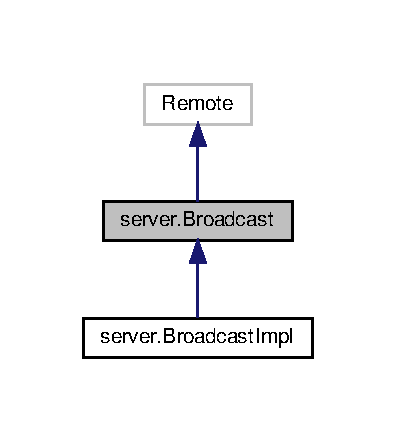
\includegraphics[width=190pt]{interfaceserver_1_1_broadcast__inherit__graph}
\end{center}
\end{figure}


Collaboration diagram for server.\+Broadcast\+:
\nopagebreak
\begin{figure}[H]
\begin{center}
\leavevmode
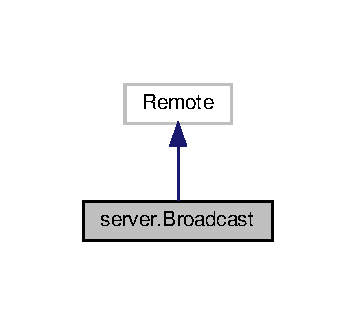
\includegraphics[width=171pt]{interfaceserver_1_1_broadcast__coll__graph}
\end{center}
\end{figure}
\subsection*{Public Member Functions}
\begin{DoxyCompactItemize}
\item 
void \hyperlink{interfaceserver_1_1_broadcast_a1a8d1242a9c00acd3347ae64debe214d}{create\+Group} (String own\+\_\+ip)  throws Remote\+Exception
\item 
void \hyperlink{interfaceserver_1_1_broadcast_a6ccaeae4c0aae1a20f1dc0c9de38abf8}{enter\+Group} (String group\+\_\+ip)  throws Remote\+Exception
\item 
\hyperlink{classstructure_1_1_group_node}{Group\+Node} \hyperlink{interfaceserver_1_1_broadcast_aac507ae95810ae722d7d204e5f0b5762}{receive\+Node} (\hyperlink{classstructure_1_1_group_node}{Group\+Node} node)  throws Remote\+Exception
\item 
Linked\+List$<$ \hyperlink{classstructure_1_1_group_node}{Group\+Node} $>$ \hyperlink{interfaceserver_1_1_broadcast_af8619fab19094de9cbc3e0b4d34eca7e}{get\+Nodes} ()  throws Remote\+Exception
\item 
void \hyperlink{interfaceserver_1_1_broadcast_a1fe00d7724fded04758454fcd1e61615}{test\+Speed} ()  throws Remote\+Exception
\item 
String \hyperlink{interfaceserver_1_1_broadcast_ad17b53d0030a03ab8262ec9c94d19cdb}{gr\+Admin} ()  throws Remote\+Exception
\item 
void \hyperlink{interfaceserver_1_1_broadcast_aaad069086f243e7b256e732a65f78763}{send\+String} (String txt, String nick, Local\+Time time, String ipF)  throws Remote\+Exception
\item 
Linked\+List$<$ \hyperlink{classstructure_1_1_message}{Message} $>$ \hyperlink{interfaceserver_1_1_broadcast_ada7537c3ca6e9d8361c7194b2a3b6e7d}{get\+M\+S\+GS} ()  throws Remote\+Exception
\item 
void \hyperlink{interfaceserver_1_1_broadcast_a96f8dad32733e1d5e503435c11e324af}{set\+M\+SG} (\hyperlink{classstructure_1_1_message}{Message} msg)  throws Remote\+Exception
\item 
\hyperlink{classstructure_1_1_group_node}{Group\+Node} \hyperlink{interfaceserver_1_1_broadcast_a16bd97cd54313805b23cb7e2255a66a6}{get\+No} ()  throws Remote\+Exception
\item 
void \hyperlink{interfaceserver_1_1_broadcast_a9efddebebb91a7da6bc0ecddcc7a32e6}{update\+Conn\+Graph} (\hyperlink{classstructure_1_1_group_node}{Group\+Node} node)  throws Remote\+Exception
\end{DoxyCompactItemize}


\subsection{Member Function Documentation}
\mbox{\Hypertarget{interfaceserver_1_1_broadcast_a1a8d1242a9c00acd3347ae64debe214d}\label{interfaceserver_1_1_broadcast_a1a8d1242a9c00acd3347ae64debe214d}} 
\index{server\+::\+Broadcast@{server\+::\+Broadcast}!create\+Group@{create\+Group}}
\index{create\+Group@{create\+Group}!server\+::\+Broadcast@{server\+::\+Broadcast}}
\subsubsection{\texorpdfstring{create\+Group()}{createGroup()}}
{\footnotesize\ttfamily void server.\+Broadcast.\+create\+Group (\begin{DoxyParamCaption}\item[{String}]{own\+\_\+ip }\end{DoxyParamCaption}) throws Remote\+Exception}



Implemented in \hyperlink{classserver_1_1_broadcast_impl_a433529db2e96faf096881d1c38033b45}{server.\+Broadcast\+Impl}.

\mbox{\Hypertarget{interfaceserver_1_1_broadcast_a6ccaeae4c0aae1a20f1dc0c9de38abf8}\label{interfaceserver_1_1_broadcast_a6ccaeae4c0aae1a20f1dc0c9de38abf8}} 
\index{server\+::\+Broadcast@{server\+::\+Broadcast}!enter\+Group@{enter\+Group}}
\index{enter\+Group@{enter\+Group}!server\+::\+Broadcast@{server\+::\+Broadcast}}
\subsubsection{\texorpdfstring{enter\+Group()}{enterGroup()}}
{\footnotesize\ttfamily void server.\+Broadcast.\+enter\+Group (\begin{DoxyParamCaption}\item[{String}]{group\+\_\+ip }\end{DoxyParamCaption}) throws Remote\+Exception}



Implemented in \hyperlink{classserver_1_1_broadcast_impl_a35a07b1f98aaaa51493cd6ff28d6b90d}{server.\+Broadcast\+Impl}.

\mbox{\Hypertarget{interfaceserver_1_1_broadcast_ada7537c3ca6e9d8361c7194b2a3b6e7d}\label{interfaceserver_1_1_broadcast_ada7537c3ca6e9d8361c7194b2a3b6e7d}} 
\index{server\+::\+Broadcast@{server\+::\+Broadcast}!get\+M\+S\+GS@{get\+M\+S\+GS}}
\index{get\+M\+S\+GS@{get\+M\+S\+GS}!server\+::\+Broadcast@{server\+::\+Broadcast}}
\subsubsection{\texorpdfstring{get\+M\+S\+G\+S()}{getMSGS()}}
{\footnotesize\ttfamily Linked\+List$<$\hyperlink{classstructure_1_1_message}{Message}$>$ server.\+Broadcast.\+get\+M\+S\+GS (\begin{DoxyParamCaption}{ }\end{DoxyParamCaption}) throws Remote\+Exception}



Implemented in \hyperlink{classserver_1_1_broadcast_impl_aecb6cd49880c2e908b1ba3d17c454ced}{server.\+Broadcast\+Impl}.

\mbox{\Hypertarget{interfaceserver_1_1_broadcast_a16bd97cd54313805b23cb7e2255a66a6}\label{interfaceserver_1_1_broadcast_a16bd97cd54313805b23cb7e2255a66a6}} 
\index{server\+::\+Broadcast@{server\+::\+Broadcast}!get\+No@{get\+No}}
\index{get\+No@{get\+No}!server\+::\+Broadcast@{server\+::\+Broadcast}}
\subsubsection{\texorpdfstring{get\+No()}{getNo()}}
{\footnotesize\ttfamily \hyperlink{classstructure_1_1_group_node}{Group\+Node} server.\+Broadcast.\+get\+No (\begin{DoxyParamCaption}{ }\end{DoxyParamCaption}) throws Remote\+Exception}



Implemented in \hyperlink{classserver_1_1_broadcast_impl_a7e004ba2fd22f9225c278f1b5bbe4dbb}{server.\+Broadcast\+Impl}.

\mbox{\Hypertarget{interfaceserver_1_1_broadcast_af8619fab19094de9cbc3e0b4d34eca7e}\label{interfaceserver_1_1_broadcast_af8619fab19094de9cbc3e0b4d34eca7e}} 
\index{server\+::\+Broadcast@{server\+::\+Broadcast}!get\+Nodes@{get\+Nodes}}
\index{get\+Nodes@{get\+Nodes}!server\+::\+Broadcast@{server\+::\+Broadcast}}
\subsubsection{\texorpdfstring{get\+Nodes()}{getNodes()}}
{\footnotesize\ttfamily Linked\+List$<$\hyperlink{classstructure_1_1_group_node}{Group\+Node}$>$ server.\+Broadcast.\+get\+Nodes (\begin{DoxyParamCaption}{ }\end{DoxyParamCaption}) throws Remote\+Exception}



Implemented in \hyperlink{classserver_1_1_broadcast_impl_aa6f1dcfe6e97de483e26a2c0a37688d3}{server.\+Broadcast\+Impl}.

\mbox{\Hypertarget{interfaceserver_1_1_broadcast_ad17b53d0030a03ab8262ec9c94d19cdb}\label{interfaceserver_1_1_broadcast_ad17b53d0030a03ab8262ec9c94d19cdb}} 
\index{server\+::\+Broadcast@{server\+::\+Broadcast}!gr\+Admin@{gr\+Admin}}
\index{gr\+Admin@{gr\+Admin}!server\+::\+Broadcast@{server\+::\+Broadcast}}
\subsubsection{\texorpdfstring{gr\+Admin()}{grAdmin()}}
{\footnotesize\ttfamily String server.\+Broadcast.\+gr\+Admin (\begin{DoxyParamCaption}{ }\end{DoxyParamCaption}) throws Remote\+Exception}



Implemented in \hyperlink{classserver_1_1_broadcast_impl_ae5995f5346d95cdbcd02361f10158671}{server.\+Broadcast\+Impl}.

\mbox{\Hypertarget{interfaceserver_1_1_broadcast_aac507ae95810ae722d7d204e5f0b5762}\label{interfaceserver_1_1_broadcast_aac507ae95810ae722d7d204e5f0b5762}} 
\index{server\+::\+Broadcast@{server\+::\+Broadcast}!receive\+Node@{receive\+Node}}
\index{receive\+Node@{receive\+Node}!server\+::\+Broadcast@{server\+::\+Broadcast}}
\subsubsection{\texorpdfstring{receive\+Node()}{receiveNode()}}
{\footnotesize\ttfamily \hyperlink{classstructure_1_1_group_node}{Group\+Node} server.\+Broadcast.\+receive\+Node (\begin{DoxyParamCaption}\item[{\hyperlink{classstructure_1_1_group_node}{Group\+Node}}]{node }\end{DoxyParamCaption}) throws Remote\+Exception}



Implemented in \hyperlink{classserver_1_1_broadcast_impl_a15437fb9a1caea537b29d0ded4809e32}{server.\+Broadcast\+Impl}.

\mbox{\Hypertarget{interfaceserver_1_1_broadcast_aaad069086f243e7b256e732a65f78763}\label{interfaceserver_1_1_broadcast_aaad069086f243e7b256e732a65f78763}} 
\index{server\+::\+Broadcast@{server\+::\+Broadcast}!send\+String@{send\+String}}
\index{send\+String@{send\+String}!server\+::\+Broadcast@{server\+::\+Broadcast}}
\subsubsection{\texorpdfstring{send\+String()}{sendString()}}
{\footnotesize\ttfamily void server.\+Broadcast.\+send\+String (\begin{DoxyParamCaption}\item[{String}]{txt,  }\item[{String}]{nick,  }\item[{Local\+Time}]{time,  }\item[{String}]{ipF }\end{DoxyParamCaption}) throws Remote\+Exception}



Implemented in \hyperlink{classserver_1_1_broadcast_impl_a5abfc6721496474d39d6b2b31589d11b}{server.\+Broadcast\+Impl}.

\mbox{\Hypertarget{interfaceserver_1_1_broadcast_a96f8dad32733e1d5e503435c11e324af}\label{interfaceserver_1_1_broadcast_a96f8dad32733e1d5e503435c11e324af}} 
\index{server\+::\+Broadcast@{server\+::\+Broadcast}!set\+M\+SG@{set\+M\+SG}}
\index{set\+M\+SG@{set\+M\+SG}!server\+::\+Broadcast@{server\+::\+Broadcast}}
\subsubsection{\texorpdfstring{set\+M\+S\+G()}{setMSG()}}
{\footnotesize\ttfamily void server.\+Broadcast.\+set\+M\+SG (\begin{DoxyParamCaption}\item[{\hyperlink{classstructure_1_1_message}{Message}}]{msg }\end{DoxyParamCaption}) throws Remote\+Exception}



Implemented in \hyperlink{classserver_1_1_broadcast_impl_a264c486f39faa2ab66a7d5a2a0c245b1}{server.\+Broadcast\+Impl}.

\mbox{\Hypertarget{interfaceserver_1_1_broadcast_a1fe00d7724fded04758454fcd1e61615}\label{interfaceserver_1_1_broadcast_a1fe00d7724fded04758454fcd1e61615}} 
\index{server\+::\+Broadcast@{server\+::\+Broadcast}!test\+Speed@{test\+Speed}}
\index{test\+Speed@{test\+Speed}!server\+::\+Broadcast@{server\+::\+Broadcast}}
\subsubsection{\texorpdfstring{test\+Speed()}{testSpeed()}}
{\footnotesize\ttfamily void server.\+Broadcast.\+test\+Speed (\begin{DoxyParamCaption}{ }\end{DoxyParamCaption}) throws Remote\+Exception}



Implemented in \hyperlink{classserver_1_1_broadcast_impl_a1ddfea5e6826ec8ff3e6aa3a3a525ccb}{server.\+Broadcast\+Impl}.

\mbox{\Hypertarget{interfaceserver_1_1_broadcast_a9efddebebb91a7da6bc0ecddcc7a32e6}\label{interfaceserver_1_1_broadcast_a9efddebebb91a7da6bc0ecddcc7a32e6}} 
\index{server\+::\+Broadcast@{server\+::\+Broadcast}!update\+Conn\+Graph@{update\+Conn\+Graph}}
\index{update\+Conn\+Graph@{update\+Conn\+Graph}!server\+::\+Broadcast@{server\+::\+Broadcast}}
\subsubsection{\texorpdfstring{update\+Conn\+Graph()}{updateConnGraph()}}
{\footnotesize\ttfamily void server.\+Broadcast.\+update\+Conn\+Graph (\begin{DoxyParamCaption}\item[{\hyperlink{classstructure_1_1_group_node}{Group\+Node}}]{node }\end{DoxyParamCaption}) throws Remote\+Exception}



Implemented in \hyperlink{classserver_1_1_broadcast_impl_abf98d794cdcf469b48cae2fbb23f1479}{server.\+Broadcast\+Impl}.



The documentation for this interface was generated from the following file\+:\begin{DoxyCompactItemize}
\item 
src/server/\hyperlink{_broadcast_8java}{Broadcast.\+java}\end{DoxyCompactItemize}

\hypertarget{classserver_1_1_broadcast_impl}{}\section{server.\+Broadcast\+Impl Class Reference}
\label{classserver_1_1_broadcast_impl}\index{server.\+Broadcast\+Impl@{server.\+Broadcast\+Impl}}


Inheritance diagram for server.\+Broadcast\+Impl\+:
\nopagebreak
\begin{figure}[H]
\begin{center}
\leavevmode
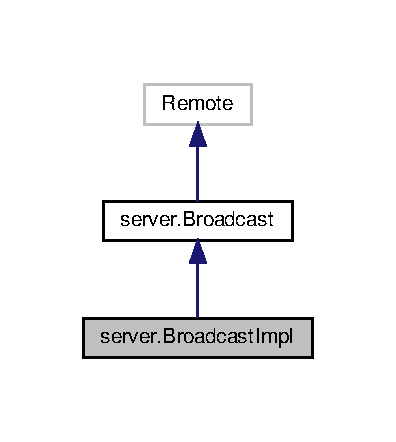
\includegraphics[width=190pt]{classserver_1_1_broadcast_impl__inherit__graph}
\end{center}
\end{figure}


Collaboration diagram for server.\+Broadcast\+Impl\+:
\nopagebreak
\begin{figure}[H]
\begin{center}
\leavevmode
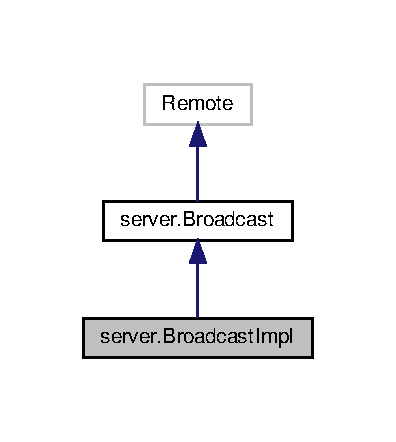
\includegraphics[width=190pt]{classserver_1_1_broadcast_impl__coll__graph}
\end{center}
\end{figure}
\subsection*{Public Member Functions}
\begin{DoxyCompactItemize}
\item 
\hyperlink{classserver_1_1_broadcast_impl_a32e3892e38d83045f927f81bca2a0ed9}{Broadcast\+Impl} ()
\item 
void \hyperlink{classserver_1_1_broadcast_impl_a433529db2e96faf096881d1c38033b45}{create\+Group} (String own\+\_\+ip)  throws Remote\+Exception 
\begin{DoxyCompactList}\small\item\em cria grupo/node \end{DoxyCompactList}\item 
void \hyperlink{classserver_1_1_broadcast_impl_a35a07b1f98aaaa51493cd6ff28d6b90d}{enter\+Group} (String group\+\_\+ip)  throws Remote\+Exception 
\begin{DoxyCompactList}\small\item\em insere um node no grupo \end{DoxyCompactList}\item 
void \hyperlink{classserver_1_1_broadcast_impl_a1ddfea5e6826ec8ff3e6aa3a3a525ccb}{test\+Speed} ()  throws Remote\+Exception 
\begin{DoxyCompactList}\small\item\em testa ping dos integrantes do grupo \end{DoxyCompactList}\item 
Linked\+List$<$ \hyperlink{classstructure_1_1_group_node}{Group\+Node} $>$ \hyperlink{classserver_1_1_broadcast_impl_aa6f1dcfe6e97de483e26a2c0a37688d3}{get\+Nodes} ()  throws Remote\+Exception 
\begin{DoxyCompactList}\small\item\em get lista de nodes do grupo \end{DoxyCompactList}\item 
\hyperlink{classstructure_1_1_group_node}{Group\+Node} \hyperlink{classserver_1_1_broadcast_impl_a15437fb9a1caea537b29d0ded4809e32}{receive\+Node} (\hyperlink{classstructure_1_1_group_node}{Group\+Node} node)  throws Remote\+Exception 
\begin{DoxyCompactList}\small\item\em Adiciona novo node. \end{DoxyCompactList}\item 
String \hyperlink{classserver_1_1_broadcast_impl_ae5995f5346d95cdbcd02361f10158671}{gr\+Admin} ()  throws Remote\+Exception
\item 
void \hyperlink{classserver_1_1_broadcast_impl_a264c486f39faa2ab66a7d5a2a0c245b1}{set\+M\+SG} (\hyperlink{classstructure_1_1_message}{Message} msg)  throws Remote\+Exception
\begin{DoxyCompactList}\small\item\em Gera relatório de conexões do grupo. \end{DoxyCompactList}\item 
\hyperlink{classstructure_1_1_group_node}{Group\+Node} \hyperlink{classserver_1_1_broadcast_impl_a7e004ba2fd22f9225c278f1b5bbe4dbb}{get\+No} ()  throws Remote\+Exception
\begin{DoxyCompactList}\small\item\em adiciona nova mensagem pendente \end{DoxyCompactList}\item 
void \hyperlink{classserver_1_1_broadcast_impl_a5abfc6721496474d39d6b2b31589d11b}{send\+String} (String txt, String nick, Local\+Time time, String ipF)  throws Remote\+Exception
\begin{DoxyCompactList}\small\item\em get node da classe \end{DoxyCompactList}\item 
Linked\+List$<$ \hyperlink{classstructure_1_1_message}{Message} $>$ \hyperlink{classserver_1_1_broadcast_impl_aecb6cd49880c2e908b1ba3d17c454ced}{get\+M\+S\+GS} ()  throws Remote\+Exception
\begin{DoxyCompactList}\small\item\em envia msgs aos outros nós que tem conexão, e assim por diante \end{DoxyCompactList}\item 
void \hyperlink{classserver_1_1_broadcast_impl_abf98d794cdcf469b48cae2fbb23f1479}{update\+Conn\+Graph} (\hyperlink{classstructure_1_1_group_node}{Group\+Node} node)  throws Remote\+Exception 
\begin{DoxyCompactList}\small\item\em retorna as mensagens recebidas \end{DoxyCompactList}\end{DoxyCompactItemize}


\subsection{Constructor \& Destructor Documentation}
\mbox{\Hypertarget{classserver_1_1_broadcast_impl_a32e3892e38d83045f927f81bca2a0ed9}\label{classserver_1_1_broadcast_impl_a32e3892e38d83045f927f81bca2a0ed9}} 
\index{server\+::\+Broadcast\+Impl@{server\+::\+Broadcast\+Impl}!Broadcast\+Impl@{Broadcast\+Impl}}
\index{Broadcast\+Impl@{Broadcast\+Impl}!server\+::\+Broadcast\+Impl@{server\+::\+Broadcast\+Impl}}
\subsubsection{\texorpdfstring{Broadcast\+Impl()}{BroadcastImpl()}}
{\footnotesize\ttfamily server.\+Broadcast\+Impl.\+Broadcast\+Impl (\begin{DoxyParamCaption}{ }\end{DoxyParamCaption})}



\subsection{Member Function Documentation}
\mbox{\Hypertarget{classserver_1_1_broadcast_impl_a433529db2e96faf096881d1c38033b45}\label{classserver_1_1_broadcast_impl_a433529db2e96faf096881d1c38033b45}} 
\index{server\+::\+Broadcast\+Impl@{server\+::\+Broadcast\+Impl}!create\+Group@{create\+Group}}
\index{create\+Group@{create\+Group}!server\+::\+Broadcast\+Impl@{server\+::\+Broadcast\+Impl}}
\subsubsection{\texorpdfstring{create\+Group()}{createGroup()}}
{\footnotesize\ttfamily public void server.\+Broadcast\+Impl.\+create\+Group (\begin{DoxyParamCaption}\item[{String}]{own\+\_\+ip }\end{DoxyParamCaption}) throws Remote\+Exception}



cria grupo/node 


\begin{DoxyParams}{Parameters}
{\em String} & own\+\_\+ip -\/ ip própria \\
\hline
\end{DoxyParams}
\begin{DoxyReturn}{Returns}
null 
\end{DoxyReturn}


Implements \hyperlink{interfaceserver_1_1_broadcast_a1a8d1242a9c00acd3347ae64debe214d}{server.\+Broadcast}.

\mbox{\Hypertarget{classserver_1_1_broadcast_impl_a35a07b1f98aaaa51493cd6ff28d6b90d}\label{classserver_1_1_broadcast_impl_a35a07b1f98aaaa51493cd6ff28d6b90d}} 
\index{server\+::\+Broadcast\+Impl@{server\+::\+Broadcast\+Impl}!enter\+Group@{enter\+Group}}
\index{enter\+Group@{enter\+Group}!server\+::\+Broadcast\+Impl@{server\+::\+Broadcast\+Impl}}
\subsubsection{\texorpdfstring{enter\+Group()}{enterGroup()}}
{\footnotesize\ttfamily public void server.\+Broadcast\+Impl.\+enter\+Group (\begin{DoxyParamCaption}\item[{String}]{group\+\_\+ip }\end{DoxyParamCaption}) throws Remote\+Exception}



insere um node no grupo 


\begin{DoxyParams}{Parameters}
{\em String} & group\+\_\+ip -\/ ip de um integrante do grupo \\
\hline
\end{DoxyParams}
\begin{DoxyReturn}{Returns}
null 
\end{DoxyReturn}


Implements \hyperlink{interfaceserver_1_1_broadcast_a6ccaeae4c0aae1a20f1dc0c9de38abf8}{server.\+Broadcast}.

\mbox{\Hypertarget{classserver_1_1_broadcast_impl_aecb6cd49880c2e908b1ba3d17c454ced}\label{classserver_1_1_broadcast_impl_aecb6cd49880c2e908b1ba3d17c454ced}} 
\index{server\+::\+Broadcast\+Impl@{server\+::\+Broadcast\+Impl}!get\+M\+S\+GS@{get\+M\+S\+GS}}
\index{get\+M\+S\+GS@{get\+M\+S\+GS}!server\+::\+Broadcast\+Impl@{server\+::\+Broadcast\+Impl}}
\subsubsection{\texorpdfstring{get\+M\+S\+G\+S()}{getMSGS()}}
{\footnotesize\ttfamily Linked\+List$<$\hyperlink{classstructure_1_1_message}{Message}$>$ server.\+Broadcast\+Impl.\+get\+M\+S\+GS (\begin{DoxyParamCaption}{ }\end{DoxyParamCaption}) throws Remote\+Exception}



envia msgs aos outros nós que tem conexão, e assim por diante 

void \hyperlink{classserver_1_1_broadcast_impl_a5abfc6721496474d39d6b2b31589d11b}{send\+String(\+String txt, String nick, Local\+Time time, String ip\+F)} throws Remote\+Exception 
\begin{DoxyParams}{Parameters}
{\em String} & txt -\/ mensagem \\
\hline
{\em String} & nick -\/ autor da mensagem \\
\hline
{\em String} & time -\/ horario de envio \\
\hline
{\em String} & ipF -\/ IP do node que está enviando a mensagem \\
\hline
\end{DoxyParams}
\begin{DoxyReturn}{Returns}
null 
\end{DoxyReturn}


Implements \hyperlink{interfaceserver_1_1_broadcast_ada7537c3ca6e9d8361c7194b2a3b6e7d}{server.\+Broadcast}.

\mbox{\Hypertarget{classserver_1_1_broadcast_impl_a7e004ba2fd22f9225c278f1b5bbe4dbb}\label{classserver_1_1_broadcast_impl_a7e004ba2fd22f9225c278f1b5bbe4dbb}} 
\index{server\+::\+Broadcast\+Impl@{server\+::\+Broadcast\+Impl}!get\+No@{get\+No}}
\index{get\+No@{get\+No}!server\+::\+Broadcast\+Impl@{server\+::\+Broadcast\+Impl}}
\subsubsection{\texorpdfstring{get\+No()}{getNo()}}
{\footnotesize\ttfamily \hyperlink{classstructure_1_1_group_node}{Group\+Node} server.\+Broadcast\+Impl.\+get\+No (\begin{DoxyParamCaption}{ }\end{DoxyParamCaption}) throws Remote\+Exception}



adiciona nova mensagem pendente 

void \hyperlink{classserver_1_1_broadcast_impl_a264c486f39faa2ab66a7d5a2a0c245b1}{set\+M\+S\+G(\+Message msg)} throws Remote\+Exception 
\begin{DoxyParams}{Parameters}
{\em Message} & msg -\/ mensagem recebida \\
\hline
\end{DoxyParams}
\begin{DoxyReturn}{Returns}
null 
\end{DoxyReturn}


Implements \hyperlink{interfaceserver_1_1_broadcast_a16bd97cd54313805b23cb7e2255a66a6}{server.\+Broadcast}.

\mbox{\Hypertarget{classserver_1_1_broadcast_impl_aa6f1dcfe6e97de483e26a2c0a37688d3}\label{classserver_1_1_broadcast_impl_aa6f1dcfe6e97de483e26a2c0a37688d3}} 
\index{server\+::\+Broadcast\+Impl@{server\+::\+Broadcast\+Impl}!get\+Nodes@{get\+Nodes}}
\index{get\+Nodes@{get\+Nodes}!server\+::\+Broadcast\+Impl@{server\+::\+Broadcast\+Impl}}
\subsubsection{\texorpdfstring{get\+Nodes()}{getNodes()}}
{\footnotesize\ttfamily public Linked\+List$<$ \hyperlink{classstructure_1_1_group_node}{Group\+Node} $>$ server.\+Broadcast\+Impl.\+get\+Nodes (\begin{DoxyParamCaption}{ }\end{DoxyParamCaption}) throws Remote\+Exception}



get lista de nodes do grupo 


\begin{DoxyParams}{Parameters}
{\em null} & \\
\hline
\end{DoxyParams}
\begin{DoxyReturn}{Returns}
Linked\+List$<$\+Group\+Node$>$ -\/ lista de nodes do grupo 
\end{DoxyReturn}


Implements \hyperlink{interfaceserver_1_1_broadcast_af8619fab19094de9cbc3e0b4d34eca7e}{server.\+Broadcast}.

\mbox{\Hypertarget{classserver_1_1_broadcast_impl_ae5995f5346d95cdbcd02361f10158671}\label{classserver_1_1_broadcast_impl_ae5995f5346d95cdbcd02361f10158671}} 
\index{server\+::\+Broadcast\+Impl@{server\+::\+Broadcast\+Impl}!gr\+Admin@{gr\+Admin}}
\index{gr\+Admin@{gr\+Admin}!server\+::\+Broadcast\+Impl@{server\+::\+Broadcast\+Impl}}
\subsubsection{\texorpdfstring{gr\+Admin()}{grAdmin()}}
{\footnotesize\ttfamily String server.\+Broadcast\+Impl.\+gr\+Admin (\begin{DoxyParamCaption}{ }\end{DoxyParamCaption}) throws Remote\+Exception}



Implements \hyperlink{interfaceserver_1_1_broadcast_ad17b53d0030a03ab8262ec9c94d19cdb}{server.\+Broadcast}.

\mbox{\Hypertarget{classserver_1_1_broadcast_impl_a15437fb9a1caea537b29d0ded4809e32}\label{classserver_1_1_broadcast_impl_a15437fb9a1caea537b29d0ded4809e32}} 
\index{server\+::\+Broadcast\+Impl@{server\+::\+Broadcast\+Impl}!receive\+Node@{receive\+Node}}
\index{receive\+Node@{receive\+Node}!server\+::\+Broadcast\+Impl@{server\+::\+Broadcast\+Impl}}
\subsubsection{\texorpdfstring{receive\+Node()}{receiveNode()}}
{\footnotesize\ttfamily public \hyperlink{classstructure_1_1_group_node}{Group\+Node} server.\+Broadcast\+Impl.\+receive\+Node (\begin{DoxyParamCaption}\item[{\hyperlink{classstructure_1_1_group_node}{Group\+Node}}]{node }\end{DoxyParamCaption}) throws Remote\+Exception}



Adiciona novo node. 


\begin{DoxyParams}{Parameters}
{\em Group\+Node} & node \\
\hline
\end{DoxyParams}
\begin{DoxyReturn}{Returns}
Group\+Node node 
\end{DoxyReturn}


Implements \hyperlink{interfaceserver_1_1_broadcast_aac507ae95810ae722d7d204e5f0b5762}{server.\+Broadcast}.

\mbox{\Hypertarget{classserver_1_1_broadcast_impl_a5abfc6721496474d39d6b2b31589d11b}\label{classserver_1_1_broadcast_impl_a5abfc6721496474d39d6b2b31589d11b}} 
\index{server\+::\+Broadcast\+Impl@{server\+::\+Broadcast\+Impl}!send\+String@{send\+String}}
\index{send\+String@{send\+String}!server\+::\+Broadcast\+Impl@{server\+::\+Broadcast\+Impl}}
\subsubsection{\texorpdfstring{send\+String()}{sendString()}}
{\footnotesize\ttfamily void server.\+Broadcast\+Impl.\+send\+String (\begin{DoxyParamCaption}\item[{String}]{txt,  }\item[{String}]{nick,  }\item[{Local\+Time}]{time,  }\item[{String}]{ipF }\end{DoxyParamCaption}) throws Remote\+Exception}



get node da classe 

Group\+Node \hyperlink{classserver_1_1_broadcast_impl_a7e004ba2fd22f9225c278f1b5bbe4dbb}{get\+No()} throws Remote\+Exception 
\begin{DoxyParams}{Parameters}
{\em null} & \\
\hline
\end{DoxyParams}
\begin{DoxyReturn}{Returns}
Group\+Node node -\/ current node 
\end{DoxyReturn}


Implements \hyperlink{interfaceserver_1_1_broadcast_aaad069086f243e7b256e732a65f78763}{server.\+Broadcast}.

\mbox{\Hypertarget{classserver_1_1_broadcast_impl_a264c486f39faa2ab66a7d5a2a0c245b1}\label{classserver_1_1_broadcast_impl_a264c486f39faa2ab66a7d5a2a0c245b1}} 
\index{server\+::\+Broadcast\+Impl@{server\+::\+Broadcast\+Impl}!set\+M\+SG@{set\+M\+SG}}
\index{set\+M\+SG@{set\+M\+SG}!server\+::\+Broadcast\+Impl@{server\+::\+Broadcast\+Impl}}
\subsubsection{\texorpdfstring{set\+M\+S\+G()}{setMSG()}}
{\footnotesize\ttfamily void server.\+Broadcast\+Impl.\+set\+M\+SG (\begin{DoxyParamCaption}\item[{\hyperlink{classstructure_1_1_message}{Message}}]{msg }\end{DoxyParamCaption}) throws Remote\+Exception}



Gera relatório de conexões do grupo. 

String \hyperlink{classserver_1_1_broadcast_impl_ae5995f5346d95cdbcd02361f10158671}{gr\+Admin()} throws Remote\+Exception 
\begin{DoxyParams}{Parameters}
{\em null} & \\
\hline
\end{DoxyParams}
\begin{DoxyReturn}{Returns}
String info -\/ numero de nós, Ip dos nós e conexões do grupo 
\end{DoxyReturn}


Implements \hyperlink{interfaceserver_1_1_broadcast_a96f8dad32733e1d5e503435c11e324af}{server.\+Broadcast}.

\mbox{\Hypertarget{classserver_1_1_broadcast_impl_a1ddfea5e6826ec8ff3e6aa3a3a525ccb}\label{classserver_1_1_broadcast_impl_a1ddfea5e6826ec8ff3e6aa3a3a525ccb}} 
\index{server\+::\+Broadcast\+Impl@{server\+::\+Broadcast\+Impl}!test\+Speed@{test\+Speed}}
\index{test\+Speed@{test\+Speed}!server\+::\+Broadcast\+Impl@{server\+::\+Broadcast\+Impl}}
\subsubsection{\texorpdfstring{test\+Speed()}{testSpeed()}}
{\footnotesize\ttfamily public void server.\+Broadcast\+Impl.\+test\+Speed (\begin{DoxyParamCaption}{ }\end{DoxyParamCaption}) throws Remote\+Exception}



testa ping dos integrantes do grupo 


\begin{DoxyParams}{Parameters}
{\em null} & \\
\hline
\end{DoxyParams}
\begin{DoxyReturn}{Returns}
null 
\end{DoxyReturn}


Implements \hyperlink{interfaceserver_1_1_broadcast_a1fe00d7724fded04758454fcd1e61615}{server.\+Broadcast}.

\mbox{\Hypertarget{classserver_1_1_broadcast_impl_abf98d794cdcf469b48cae2fbb23f1479}\label{classserver_1_1_broadcast_impl_abf98d794cdcf469b48cae2fbb23f1479}} 
\index{server\+::\+Broadcast\+Impl@{server\+::\+Broadcast\+Impl}!update\+Conn\+Graph@{update\+Conn\+Graph}}
\index{update\+Conn\+Graph@{update\+Conn\+Graph}!server\+::\+Broadcast\+Impl@{server\+::\+Broadcast\+Impl}}
\subsubsection{\texorpdfstring{update\+Conn\+Graph()}{updateConnGraph()}}
{\footnotesize\ttfamily void server.\+Broadcast\+Impl.\+update\+Conn\+Graph (\begin{DoxyParamCaption}\item[{\hyperlink{classstructure_1_1_group_node}{Group\+Node}}]{node }\end{DoxyParamCaption}) throws Remote\+Exception}



retorna as mensagens recebidas 

public Linked\+List$<$\+Message$>$ \hyperlink{classserver_1_1_broadcast_impl_aecb6cd49880c2e908b1ba3d17c454ced}{get\+M\+S\+G\+S()} throws Remote\+Exception 
\begin{DoxyParams}{Parameters}
{\em null} & \\
\hline
\end{DoxyParams}
\begin{DoxyReturn}{Returns}
Linked\+List$<$\+Message$>$ 
\end{DoxyReturn}


Implements \hyperlink{interfaceserver_1_1_broadcast_a9efddebebb91a7da6bc0ecddcc7a32e6}{server.\+Broadcast}.



The documentation for this class was generated from the following file\+:\begin{DoxyCompactItemize}
\item 
src/server/\hyperlink{_broadcast_impl_8java}{Broadcast\+Impl.\+java}\end{DoxyCompactItemize}

\hypertarget{classstructure_1_1_client_tela}{}\section{structure.\+Client\+Tela Class Reference}
\label{classstructure_1_1_client_tela}\index{structure.\+Client\+Tela@{structure.\+Client\+Tela}}


Collaboration diagram for structure.\+Client\+Tela\+:
\nopagebreak
\begin{figure}[H]
\begin{center}
\leavevmode
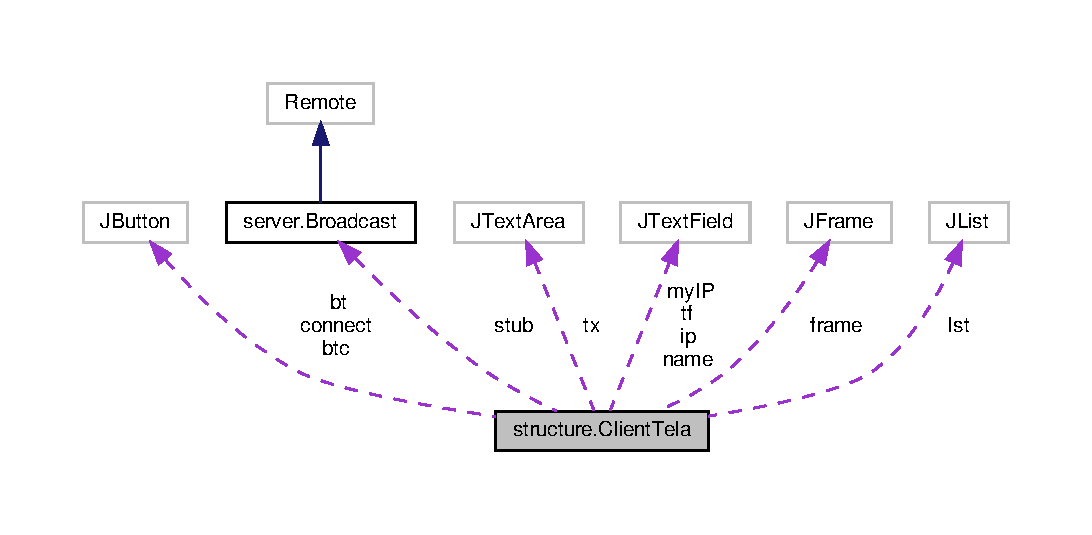
\includegraphics[width=350pt]{classstructure_1_1_client_tela__coll__graph}
\end{center}
\end{figure}
\subsection*{Public Member Functions}
\begin{DoxyCompactItemize}
\item 
void \hyperlink{classstructure_1_1_client_tela_a60fdbdd395b62d73b5bdeac95237fcc0}{do\+Connect} ()
\begin{DoxyCompactList}\small\item\em chama a conexão do usuario do usuario ao grupo \end{DoxyCompactList}\item 
void \hyperlink{classstructure_1_1_client_tela_a7b102bb8543266eed71ff94ac46fd815}{send\+Text} ()
\begin{DoxyCompactList}\small\item\em envia mensagens \end{DoxyCompactList}\item 
void \hyperlink{classstructure_1_1_client_tela_a7b9558eff45ebd37710065d2607329fb}{close\+Connection} ()
\begin{DoxyCompactList}\small\item\em chama processo de saida do grupo \end{DoxyCompactList}\item 
\hyperlink{classstructure_1_1_client_tela_a0f805fc16d6609f1063575f445ee5a56}{Client\+Tela} ()
\end{DoxyCompactItemize}
\subsection*{Static Public Member Functions}
\begin{DoxyCompactItemize}
\item 
static void \hyperlink{classstructure_1_1_client_tela_ab70271ebd978b7bf287b1f18d4febae7}{main} (String\mbox{[}$\,$\mbox{]} args)
\begin{DoxyCompactList}\small\item\em inicializa o app \end{DoxyCompactList}\end{DoxyCompactItemize}


\subsection{Constructor \& Destructor Documentation}
\mbox{\Hypertarget{classstructure_1_1_client_tela_a0f805fc16d6609f1063575f445ee5a56}\label{classstructure_1_1_client_tela_a0f805fc16d6609f1063575f445ee5a56}} 
\index{structure\+::\+Client\+Tela@{structure\+::\+Client\+Tela}!Client\+Tela@{Client\+Tela}}
\index{Client\+Tela@{Client\+Tela}!structure\+::\+Client\+Tela@{structure\+::\+Client\+Tela}}
\subsubsection{\texorpdfstring{Client\+Tela()}{ClientTela()}}
{\footnotesize\ttfamily structure.\+Client\+Tela.\+Client\+Tela (\begin{DoxyParamCaption}{ }\end{DoxyParamCaption})}



\subsection{Member Function Documentation}
\mbox{\Hypertarget{classstructure_1_1_client_tela_a7b9558eff45ebd37710065d2607329fb}\label{classstructure_1_1_client_tela_a7b9558eff45ebd37710065d2607329fb}} 
\index{structure\+::\+Client\+Tela@{structure\+::\+Client\+Tela}!close\+Connection@{close\+Connection}}
\index{close\+Connection@{close\+Connection}!structure\+::\+Client\+Tela@{structure\+::\+Client\+Tela}}
\subsubsection{\texorpdfstring{close\+Connection()}{closeConnection()}}
{\footnotesize\ttfamily public void structure.\+Client\+Tela.\+close\+Connection (\begin{DoxyParamCaption}{ }\end{DoxyParamCaption})}



chama processo de saida do grupo 


\begin{DoxyParams}{Parameters}
{\em null} & \\
\hline
\end{DoxyParams}
\begin{DoxyReturn}{Returns}
null 
\end{DoxyReturn}
\mbox{\Hypertarget{classstructure_1_1_client_tela_a60fdbdd395b62d73b5bdeac95237fcc0}\label{classstructure_1_1_client_tela_a60fdbdd395b62d73b5bdeac95237fcc0}} 
\index{structure\+::\+Client\+Tela@{structure\+::\+Client\+Tela}!do\+Connect@{do\+Connect}}
\index{do\+Connect@{do\+Connect}!structure\+::\+Client\+Tela@{structure\+::\+Client\+Tela}}
\subsubsection{\texorpdfstring{do\+Connect()}{doConnect()}}
{\footnotesize\ttfamily public void structure.\+Client\+Tela.\+do\+Connect (\begin{DoxyParamCaption}{ }\end{DoxyParamCaption})}



chama a conexão do usuario do usuario ao grupo 


\begin{DoxyParams}{Parameters}
{\em null} & \\
\hline
\end{DoxyParams}
\begin{DoxyReturn}{Returns}
null 
\end{DoxyReturn}
\mbox{\Hypertarget{classstructure_1_1_client_tela_ab70271ebd978b7bf287b1f18d4febae7}\label{classstructure_1_1_client_tela_ab70271ebd978b7bf287b1f18d4febae7}} 
\index{structure\+::\+Client\+Tela@{structure\+::\+Client\+Tela}!main@{main}}
\index{main@{main}!structure\+::\+Client\+Tela@{structure\+::\+Client\+Tela}}
\subsubsection{\texorpdfstring{main()}{main()}}
{\footnotesize\ttfamily public static void structure.\+Client\+Tela.\+main (\begin{DoxyParamCaption}\item[{String \mbox{[}$\,$\mbox{]}}]{args }\end{DoxyParamCaption})\hspace{0.3cm}{\ttfamily [static]}}



inicializa o app 


\begin{DoxyParams}{Parameters}
{\em null} & \\
\hline
\end{DoxyParams}
\begin{DoxyReturn}{Returns}
null 
\end{DoxyReturn}
\mbox{\Hypertarget{classstructure_1_1_client_tela_a7b102bb8543266eed71ff94ac46fd815}\label{classstructure_1_1_client_tela_a7b102bb8543266eed71ff94ac46fd815}} 
\index{structure\+::\+Client\+Tela@{structure\+::\+Client\+Tela}!send\+Text@{send\+Text}}
\index{send\+Text@{send\+Text}!structure\+::\+Client\+Tela@{structure\+::\+Client\+Tela}}
\subsubsection{\texorpdfstring{send\+Text()}{sendText()}}
{\footnotesize\ttfamily public void structure.\+Client\+Tela.\+send\+Text (\begin{DoxyParamCaption}{ }\end{DoxyParamCaption})}



envia mensagens 


\begin{DoxyParams}{Parameters}
{\em null} & \\
\hline
\end{DoxyParams}
\begin{DoxyReturn}{Returns}
null 
\end{DoxyReturn}


The documentation for this class was generated from the following file\+:\begin{DoxyCompactItemize}
\item 
src/structure/\hyperlink{_client_tela_8java}{Client\+Tela.\+java}\end{DoxyCompactItemize}

\hypertarget{classstructure_1_1_connection_graph}{}\section{structure.\+Connection\+Graph Class Reference}
\label{classstructure_1_1_connection_graph}\index{structure.\+Connection\+Graph@{structure.\+Connection\+Graph}}


Inheritance diagram for structure.\+Connection\+Graph\+:
\nopagebreak
\begin{figure}[H]
\begin{center}
\leavevmode
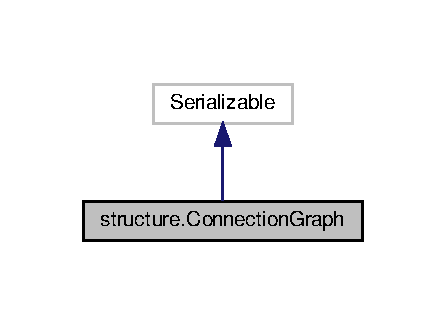
\includegraphics[width=214pt]{classstructure_1_1_connection_graph__inherit__graph}
\end{center}
\end{figure}


Collaboration diagram for structure.\+Connection\+Graph\+:
\nopagebreak
\begin{figure}[H]
\begin{center}
\leavevmode
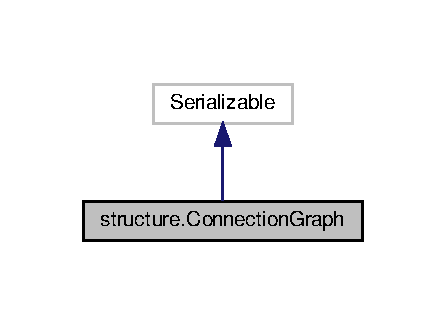
\includegraphics[width=214pt]{classstructure_1_1_connection_graph__coll__graph}
\end{center}
\end{figure}
\subsection*{Public Member Functions}
\begin{DoxyCompactItemize}
\item 
\hyperlink{classstructure_1_1_connection_graph_a1af2e60866156900889b166760fe0a78}{Connection\+Graph} ()
\item 
Hash\+Map$<$ Integer, Linked\+List$<$ \hyperlink{classstructure_1_1_group_node}{Group\+Node} $>$ $>$ \hyperlink{classstructure_1_1_connection_graph_ac09bdf474306cbfb1aee7404c7d74e80}{get\+Connections} ()
\item 
void \hyperlink{classstructure_1_1_connection_graph_a96375503c72465740c4919c207619744}{merge} (\hyperlink{classstructure_1_1_connection_graph}{Connection\+Graph} connections)
\item 
void \hyperlink{classstructure_1_1_connection_graph_afc71ae9bd27880a4854fa69d8cbbebc3}{add\+Connection} (Integer id, \hyperlink{classstructure_1_1_group_node}{Group\+Node} node)
\item 
Linked\+List$<$ \hyperlink{classstructure_1_1_group_node}{Group\+Node} $>$ \hyperlink{classstructure_1_1_connection_graph_a6f2466c51efe95a9422e667631af59e8}{get\+Nodes} ()
\item 
void \hyperlink{classstructure_1_1_connection_graph_aab26e85cf3048c1682a6552624d5436c}{add\+Node} (\hyperlink{classstructure_1_1_group_node}{Group\+Node} node)
\item 
boolean \hyperlink{classstructure_1_1_connection_graph_ad86b7fa7e8a3e7206c6ca7b4aee96536}{equals} (Object o)
\item 
int \hyperlink{classstructure_1_1_connection_graph_af352a3e79444b178fc8edef545086836}{hash\+Code} ()
\item 
String \hyperlink{classstructure_1_1_connection_graph_afa0d01d543f0f89f713a3825cf14521e}{to\+String} ()
\end{DoxyCompactItemize}


\subsection{Constructor \& Destructor Documentation}
\mbox{\Hypertarget{classstructure_1_1_connection_graph_a1af2e60866156900889b166760fe0a78}\label{classstructure_1_1_connection_graph_a1af2e60866156900889b166760fe0a78}} 
\index{structure\+::\+Connection\+Graph@{structure\+::\+Connection\+Graph}!Connection\+Graph@{Connection\+Graph}}
\index{Connection\+Graph@{Connection\+Graph}!structure\+::\+Connection\+Graph@{structure\+::\+Connection\+Graph}}
\subsubsection{\texorpdfstring{Connection\+Graph()}{ConnectionGraph()}}
{\footnotesize\ttfamily structure.\+Connection\+Graph.\+Connection\+Graph (\begin{DoxyParamCaption}{ }\end{DoxyParamCaption})}



\subsection{Member Function Documentation}
\mbox{\Hypertarget{classstructure_1_1_connection_graph_afc71ae9bd27880a4854fa69d8cbbebc3}\label{classstructure_1_1_connection_graph_afc71ae9bd27880a4854fa69d8cbbebc3}} 
\index{structure\+::\+Connection\+Graph@{structure\+::\+Connection\+Graph}!add\+Connection@{add\+Connection}}
\index{add\+Connection@{add\+Connection}!structure\+::\+Connection\+Graph@{structure\+::\+Connection\+Graph}}
\subsubsection{\texorpdfstring{add\+Connection()}{addConnection()}}
{\footnotesize\ttfamily void structure.\+Connection\+Graph.\+add\+Connection (\begin{DoxyParamCaption}\item[{Integer}]{id,  }\item[{\hyperlink{classstructure_1_1_group_node}{Group\+Node}}]{node }\end{DoxyParamCaption})}

\mbox{\Hypertarget{classstructure_1_1_connection_graph_aab26e85cf3048c1682a6552624d5436c}\label{classstructure_1_1_connection_graph_aab26e85cf3048c1682a6552624d5436c}} 
\index{structure\+::\+Connection\+Graph@{structure\+::\+Connection\+Graph}!add\+Node@{add\+Node}}
\index{add\+Node@{add\+Node}!structure\+::\+Connection\+Graph@{structure\+::\+Connection\+Graph}}
\subsubsection{\texorpdfstring{add\+Node()}{addNode()}}
{\footnotesize\ttfamily void structure.\+Connection\+Graph.\+add\+Node (\begin{DoxyParamCaption}\item[{\hyperlink{classstructure_1_1_group_node}{Group\+Node}}]{node }\end{DoxyParamCaption})}

\mbox{\Hypertarget{classstructure_1_1_connection_graph_ad86b7fa7e8a3e7206c6ca7b4aee96536}\label{classstructure_1_1_connection_graph_ad86b7fa7e8a3e7206c6ca7b4aee96536}} 
\index{structure\+::\+Connection\+Graph@{structure\+::\+Connection\+Graph}!equals@{equals}}
\index{equals@{equals}!structure\+::\+Connection\+Graph@{structure\+::\+Connection\+Graph}}
\subsubsection{\texorpdfstring{equals()}{equals()}}
{\footnotesize\ttfamily boolean structure.\+Connection\+Graph.\+equals (\begin{DoxyParamCaption}\item[{Object}]{o }\end{DoxyParamCaption})}

\mbox{\Hypertarget{classstructure_1_1_connection_graph_ac09bdf474306cbfb1aee7404c7d74e80}\label{classstructure_1_1_connection_graph_ac09bdf474306cbfb1aee7404c7d74e80}} 
\index{structure\+::\+Connection\+Graph@{structure\+::\+Connection\+Graph}!get\+Connections@{get\+Connections}}
\index{get\+Connections@{get\+Connections}!structure\+::\+Connection\+Graph@{structure\+::\+Connection\+Graph}}
\subsubsection{\texorpdfstring{get\+Connections()}{getConnections()}}
{\footnotesize\ttfamily Hash\+Map$<$Integer,Linked\+List$<$\hyperlink{classstructure_1_1_group_node}{Group\+Node}$>$ $>$ structure.\+Connection\+Graph.\+get\+Connections (\begin{DoxyParamCaption}{ }\end{DoxyParamCaption})}

\mbox{\Hypertarget{classstructure_1_1_connection_graph_a6f2466c51efe95a9422e667631af59e8}\label{classstructure_1_1_connection_graph_a6f2466c51efe95a9422e667631af59e8}} 
\index{structure\+::\+Connection\+Graph@{structure\+::\+Connection\+Graph}!get\+Nodes@{get\+Nodes}}
\index{get\+Nodes@{get\+Nodes}!structure\+::\+Connection\+Graph@{structure\+::\+Connection\+Graph}}
\subsubsection{\texorpdfstring{get\+Nodes()}{getNodes()}}
{\footnotesize\ttfamily Linked\+List$<$\hyperlink{classstructure_1_1_group_node}{Group\+Node}$>$ structure.\+Connection\+Graph.\+get\+Nodes (\begin{DoxyParamCaption}{ }\end{DoxyParamCaption})}

\mbox{\Hypertarget{classstructure_1_1_connection_graph_af352a3e79444b178fc8edef545086836}\label{classstructure_1_1_connection_graph_af352a3e79444b178fc8edef545086836}} 
\index{structure\+::\+Connection\+Graph@{structure\+::\+Connection\+Graph}!hash\+Code@{hash\+Code}}
\index{hash\+Code@{hash\+Code}!structure\+::\+Connection\+Graph@{structure\+::\+Connection\+Graph}}
\subsubsection{\texorpdfstring{hash\+Code()}{hashCode()}}
{\footnotesize\ttfamily int structure.\+Connection\+Graph.\+hash\+Code (\begin{DoxyParamCaption}{ }\end{DoxyParamCaption})}

\mbox{\Hypertarget{classstructure_1_1_connection_graph_a96375503c72465740c4919c207619744}\label{classstructure_1_1_connection_graph_a96375503c72465740c4919c207619744}} 
\index{structure\+::\+Connection\+Graph@{structure\+::\+Connection\+Graph}!merge@{merge}}
\index{merge@{merge}!structure\+::\+Connection\+Graph@{structure\+::\+Connection\+Graph}}
\subsubsection{\texorpdfstring{merge()}{merge()}}
{\footnotesize\ttfamily void structure.\+Connection\+Graph.\+merge (\begin{DoxyParamCaption}\item[{\hyperlink{classstructure_1_1_connection_graph}{Connection\+Graph}}]{connections }\end{DoxyParamCaption})}

\mbox{\Hypertarget{classstructure_1_1_connection_graph_afa0d01d543f0f89f713a3825cf14521e}\label{classstructure_1_1_connection_graph_afa0d01d543f0f89f713a3825cf14521e}} 
\index{structure\+::\+Connection\+Graph@{structure\+::\+Connection\+Graph}!to\+String@{to\+String}}
\index{to\+String@{to\+String}!structure\+::\+Connection\+Graph@{structure\+::\+Connection\+Graph}}
\subsubsection{\texorpdfstring{to\+String()}{toString()}}
{\footnotesize\ttfamily String structure.\+Connection\+Graph.\+to\+String (\begin{DoxyParamCaption}{ }\end{DoxyParamCaption})}



The documentation for this class was generated from the following file\+:\begin{DoxyCompactItemize}
\item 
src/structure/\hyperlink{_connection_graph_8java}{Connection\+Graph.\+java}\end{DoxyCompactItemize}

\hypertarget{classserver_1_1gr_admin}{}\section{server.\+gr\+Admin Class Reference}
\label{classserver_1_1gr_admin}\index{server.\+gr\+Admin@{server.\+gr\+Admin}}
\subsection*{Static Public Member Functions}
\begin{DoxyCompactItemize}
\item 
static void \hyperlink{classserver_1_1gr_admin_a4bde363e4e636eb9ef8e4ee55a1857d8}{main} (String\mbox{[}$\,$\mbox{]} args)
\begin{DoxyCompactList}\small\item\em se conecta com um nó e exibe as infos de admin dele \end{DoxyCompactList}\end{DoxyCompactItemize}


\subsection{Member Function Documentation}
\mbox{\Hypertarget{classserver_1_1gr_admin_a4bde363e4e636eb9ef8e4ee55a1857d8}\label{classserver_1_1gr_admin_a4bde363e4e636eb9ef8e4ee55a1857d8}} 
\index{server\+::gr\+Admin@{server\+::gr\+Admin}!main@{main}}
\index{main@{main}!server\+::gr\+Admin@{server\+::gr\+Admin}}
\subsubsection{\texorpdfstring{main()}{main()}}
{\footnotesize\ttfamily public static void server.\+gr\+Admin.\+main (\begin{DoxyParamCaption}\item[{String \mbox{[}$\,$\mbox{]}}]{args }\end{DoxyParamCaption})\hspace{0.3cm}{\ttfamily [static]}}



se conecta com um nó e exibe as infos de admin dele 


\begin{DoxyParams}{Parameters}
{\em null} & \\
\hline
\end{DoxyParams}
\begin{DoxyReturn}{Returns}
null 
\end{DoxyReturn}


The documentation for this class was generated from the following file\+:\begin{DoxyCompactItemize}
\item 
src/server/\hyperlink{gr_admin_8java}{gr\+Admin.\+java}\end{DoxyCompactItemize}

\hypertarget{classstructure_1_1_group_node}{}\section{structure.\+Group\+Node Class Reference}
\label{classstructure_1_1_group_node}\index{structure.\+Group\+Node@{structure.\+Group\+Node}}


Inheritance diagram for structure.\+Group\+Node\+:
\nopagebreak
\begin{figure}[H]
\begin{center}
\leavevmode
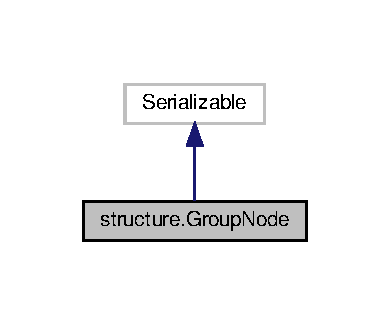
\includegraphics[width=187pt]{classstructure_1_1_group_node__inherit__graph}
\end{center}
\end{figure}


Collaboration diagram for structure.\+Group\+Node\+:
\nopagebreak
\begin{figure}[H]
\begin{center}
\leavevmode
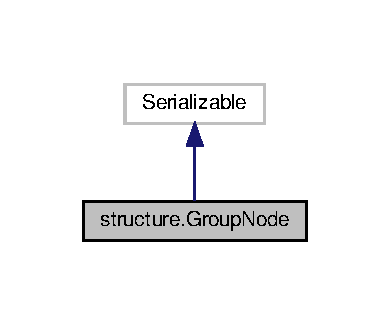
\includegraphics[width=187pt]{classstructure_1_1_group_node__coll__graph}
\end{center}
\end{figure}
\subsection*{Public Member Functions}
\begin{DoxyCompactItemize}
\item 
\hyperlink{classstructure_1_1_group_node_a22c95192d00d8f968102e79bee9b55d9}{Group\+Node} (String IP)
\item 
void \hyperlink{classstructure_1_1_group_node_a328fa38c77c507d7a6a4d36984cf0022}{set\+Stub1} (\hyperlink{interfaceserver_1_1_broadcast}{Broadcast} stub)
\item 
void \hyperlink{classstructure_1_1_group_node_a6baa802bddde09ff85c44fd92200b058}{set\+Stub2} (\hyperlink{interfaceserver_1_1_broadcast}{Broadcast} stub)
\item 
void \hyperlink{classstructure_1_1_group_node_a8195f402759827e1a5d179fad08a60d8}{set\+Stub3} (\hyperlink{interfaceserver_1_1_broadcast}{Broadcast} stub)
\item 
\hyperlink{interfaceserver_1_1_broadcast}{Broadcast} \hyperlink{classstructure_1_1_group_node_a60db881a161932baf99076509258eb50}{get\+Stub1} ()
\item 
\hyperlink{interfaceserver_1_1_broadcast}{Broadcast} \hyperlink{classstructure_1_1_group_node_a39de0cad8c3e43e938482c74683a291d}{get\+Stub2} ()
\item 
\hyperlink{interfaceserver_1_1_broadcast}{Broadcast} \hyperlink{classstructure_1_1_group_node_ac9b11b128f621dc8784dccc4fb5ceae1}{get\+Stub3} ()
\item 
String \hyperlink{classstructure_1_1_group_node_ac2f64cbb8eb9332df8663e80e1bb3f61}{get\+IP} ()
\item 
void \hyperlink{classstructure_1_1_group_node_a0baf2a9e22ec4685e7394a5f3d87a810}{set\+IP} (String IP)
\item 
int \hyperlink{classstructure_1_1_group_node_afb3b82694003309b6218f908110838c6}{get\+ID} ()
\item 
void \hyperlink{classstructure_1_1_group_node_af109d88d565e87b1da693278d504107a}{set\+ID} (int ID)
\item 
Linked\+List$<$ \hyperlink{classstructure_1_1_message}{Message} $>$ \hyperlink{classstructure_1_1_group_node_a8a0df6e9ac4997341fa90e3b844e8176}{get\+Messages} ()
\item 
void \hyperlink{classstructure_1_1_group_node_a0b6f67a6194009da3bca009c395e8f7a}{add\+Message} (\hyperlink{classstructure_1_1_message}{Message} msg)
\item 
\hyperlink{classstructure_1_1_connection_graph}{Connection\+Graph} \hyperlink{classstructure_1_1_group_node_a13b5457f1b989a0aa8da6440610882fb}{get\+Connections} ()
\item 
void \hyperlink{classstructure_1_1_group_node_acd052974ff110c595e1ab115460a08c4}{add\+Connection} (\hyperlink{classstructure_1_1_group_node}{Group\+Node} node)
\item 
void \hyperlink{classstructure_1_1_group_node_afdecedab839a4aca2282a2ddce6290cb}{merge\+Connections} (\hyperlink{classstructure_1_1_connection_graph}{Connection\+Graph} graph)
\item 
boolean \hyperlink{classstructure_1_1_group_node_a4c529c68ff5c5a1951967a620305ce9a}{check\+Availability} ()
\item 
boolean \hyperlink{classstructure_1_1_group_node_ac13e06c08ea2141b48ce07d5e50e512e}{equals} (Object o)
\item 
int \hyperlink{classstructure_1_1_group_node_aa3e51b1b49633aa9a458dd85b2dc1629}{hash\+Code} ()
\item 
String \hyperlink{classstructure_1_1_group_node_ab0076e02c1b7c6934ee012dfd3fe94e7}{to\+String} ()
\end{DoxyCompactItemize}


\subsection{Constructor \& Destructor Documentation}
\mbox{\Hypertarget{classstructure_1_1_group_node_a22c95192d00d8f968102e79bee9b55d9}\label{classstructure_1_1_group_node_a22c95192d00d8f968102e79bee9b55d9}} 
\index{structure\+::\+Group\+Node@{structure\+::\+Group\+Node}!Group\+Node@{Group\+Node}}
\index{Group\+Node@{Group\+Node}!structure\+::\+Group\+Node@{structure\+::\+Group\+Node}}
\subsubsection{\texorpdfstring{Group\+Node()}{GroupNode()}}
{\footnotesize\ttfamily structure.\+Group\+Node.\+Group\+Node (\begin{DoxyParamCaption}\item[{String}]{IP }\end{DoxyParamCaption})}



\subsection{Member Function Documentation}
\mbox{\Hypertarget{classstructure_1_1_group_node_acd052974ff110c595e1ab115460a08c4}\label{classstructure_1_1_group_node_acd052974ff110c595e1ab115460a08c4}} 
\index{structure\+::\+Group\+Node@{structure\+::\+Group\+Node}!add\+Connection@{add\+Connection}}
\index{add\+Connection@{add\+Connection}!structure\+::\+Group\+Node@{structure\+::\+Group\+Node}}
\subsubsection{\texorpdfstring{add\+Connection()}{addConnection()}}
{\footnotesize\ttfamily void structure.\+Group\+Node.\+add\+Connection (\begin{DoxyParamCaption}\item[{\hyperlink{classstructure_1_1_group_node}{Group\+Node}}]{node }\end{DoxyParamCaption})}

\mbox{\Hypertarget{classstructure_1_1_group_node_a0b6f67a6194009da3bca009c395e8f7a}\label{classstructure_1_1_group_node_a0b6f67a6194009da3bca009c395e8f7a}} 
\index{structure\+::\+Group\+Node@{structure\+::\+Group\+Node}!add\+Message@{add\+Message}}
\index{add\+Message@{add\+Message}!structure\+::\+Group\+Node@{structure\+::\+Group\+Node}}
\subsubsection{\texorpdfstring{add\+Message()}{addMessage()}}
{\footnotesize\ttfamily void structure.\+Group\+Node.\+add\+Message (\begin{DoxyParamCaption}\item[{\hyperlink{classstructure_1_1_message}{Message}}]{msg }\end{DoxyParamCaption})}

\mbox{\Hypertarget{classstructure_1_1_group_node_a4c529c68ff5c5a1951967a620305ce9a}\label{classstructure_1_1_group_node_a4c529c68ff5c5a1951967a620305ce9a}} 
\index{structure\+::\+Group\+Node@{structure\+::\+Group\+Node}!check\+Availability@{check\+Availability}}
\index{check\+Availability@{check\+Availability}!structure\+::\+Group\+Node@{structure\+::\+Group\+Node}}
\subsubsection{\texorpdfstring{check\+Availability()}{checkAvailability()}}
{\footnotesize\ttfamily boolean structure.\+Group\+Node.\+check\+Availability (\begin{DoxyParamCaption}{ }\end{DoxyParamCaption})}

\mbox{\Hypertarget{classstructure_1_1_group_node_ac13e06c08ea2141b48ce07d5e50e512e}\label{classstructure_1_1_group_node_ac13e06c08ea2141b48ce07d5e50e512e}} 
\index{structure\+::\+Group\+Node@{structure\+::\+Group\+Node}!equals@{equals}}
\index{equals@{equals}!structure\+::\+Group\+Node@{structure\+::\+Group\+Node}}
\subsubsection{\texorpdfstring{equals()}{equals()}}
{\footnotesize\ttfamily boolean structure.\+Group\+Node.\+equals (\begin{DoxyParamCaption}\item[{Object}]{o }\end{DoxyParamCaption})}

\mbox{\Hypertarget{classstructure_1_1_group_node_a13b5457f1b989a0aa8da6440610882fb}\label{classstructure_1_1_group_node_a13b5457f1b989a0aa8da6440610882fb}} 
\index{structure\+::\+Group\+Node@{structure\+::\+Group\+Node}!get\+Connections@{get\+Connections}}
\index{get\+Connections@{get\+Connections}!structure\+::\+Group\+Node@{structure\+::\+Group\+Node}}
\subsubsection{\texorpdfstring{get\+Connections()}{getConnections()}}
{\footnotesize\ttfamily \hyperlink{classstructure_1_1_connection_graph}{Connection\+Graph} structure.\+Group\+Node.\+get\+Connections (\begin{DoxyParamCaption}{ }\end{DoxyParamCaption})}

\mbox{\Hypertarget{classstructure_1_1_group_node_afb3b82694003309b6218f908110838c6}\label{classstructure_1_1_group_node_afb3b82694003309b6218f908110838c6}} 
\index{structure\+::\+Group\+Node@{structure\+::\+Group\+Node}!get\+ID@{get\+ID}}
\index{get\+ID@{get\+ID}!structure\+::\+Group\+Node@{structure\+::\+Group\+Node}}
\subsubsection{\texorpdfstring{get\+I\+D()}{getID()}}
{\footnotesize\ttfamily int structure.\+Group\+Node.\+get\+ID (\begin{DoxyParamCaption}{ }\end{DoxyParamCaption})}

\mbox{\Hypertarget{classstructure_1_1_group_node_ac2f64cbb8eb9332df8663e80e1bb3f61}\label{classstructure_1_1_group_node_ac2f64cbb8eb9332df8663e80e1bb3f61}} 
\index{structure\+::\+Group\+Node@{structure\+::\+Group\+Node}!get\+IP@{get\+IP}}
\index{get\+IP@{get\+IP}!structure\+::\+Group\+Node@{structure\+::\+Group\+Node}}
\subsubsection{\texorpdfstring{get\+I\+P()}{getIP()}}
{\footnotesize\ttfamily String structure.\+Group\+Node.\+get\+IP (\begin{DoxyParamCaption}{ }\end{DoxyParamCaption})}

\mbox{\Hypertarget{classstructure_1_1_group_node_a8a0df6e9ac4997341fa90e3b844e8176}\label{classstructure_1_1_group_node_a8a0df6e9ac4997341fa90e3b844e8176}} 
\index{structure\+::\+Group\+Node@{structure\+::\+Group\+Node}!get\+Messages@{get\+Messages}}
\index{get\+Messages@{get\+Messages}!structure\+::\+Group\+Node@{structure\+::\+Group\+Node}}
\subsubsection{\texorpdfstring{get\+Messages()}{getMessages()}}
{\footnotesize\ttfamily Linked\+List$<$\hyperlink{classstructure_1_1_message}{Message}$>$ structure.\+Group\+Node.\+get\+Messages (\begin{DoxyParamCaption}{ }\end{DoxyParamCaption})}

\mbox{\Hypertarget{classstructure_1_1_group_node_a60db881a161932baf99076509258eb50}\label{classstructure_1_1_group_node_a60db881a161932baf99076509258eb50}} 
\index{structure\+::\+Group\+Node@{structure\+::\+Group\+Node}!get\+Stub1@{get\+Stub1}}
\index{get\+Stub1@{get\+Stub1}!structure\+::\+Group\+Node@{structure\+::\+Group\+Node}}
\subsubsection{\texorpdfstring{get\+Stub1()}{getStub1()}}
{\footnotesize\ttfamily \hyperlink{interfaceserver_1_1_broadcast}{Broadcast} structure.\+Group\+Node.\+get\+Stub1 (\begin{DoxyParamCaption}{ }\end{DoxyParamCaption})}

\mbox{\Hypertarget{classstructure_1_1_group_node_a39de0cad8c3e43e938482c74683a291d}\label{classstructure_1_1_group_node_a39de0cad8c3e43e938482c74683a291d}} 
\index{structure\+::\+Group\+Node@{structure\+::\+Group\+Node}!get\+Stub2@{get\+Stub2}}
\index{get\+Stub2@{get\+Stub2}!structure\+::\+Group\+Node@{structure\+::\+Group\+Node}}
\subsubsection{\texorpdfstring{get\+Stub2()}{getStub2()}}
{\footnotesize\ttfamily \hyperlink{interfaceserver_1_1_broadcast}{Broadcast} structure.\+Group\+Node.\+get\+Stub2 (\begin{DoxyParamCaption}{ }\end{DoxyParamCaption})}

\mbox{\Hypertarget{classstructure_1_1_group_node_ac9b11b128f621dc8784dccc4fb5ceae1}\label{classstructure_1_1_group_node_ac9b11b128f621dc8784dccc4fb5ceae1}} 
\index{structure\+::\+Group\+Node@{structure\+::\+Group\+Node}!get\+Stub3@{get\+Stub3}}
\index{get\+Stub3@{get\+Stub3}!structure\+::\+Group\+Node@{structure\+::\+Group\+Node}}
\subsubsection{\texorpdfstring{get\+Stub3()}{getStub3()}}
{\footnotesize\ttfamily \hyperlink{interfaceserver_1_1_broadcast}{Broadcast} structure.\+Group\+Node.\+get\+Stub3 (\begin{DoxyParamCaption}{ }\end{DoxyParamCaption})}

\mbox{\Hypertarget{classstructure_1_1_group_node_aa3e51b1b49633aa9a458dd85b2dc1629}\label{classstructure_1_1_group_node_aa3e51b1b49633aa9a458dd85b2dc1629}} 
\index{structure\+::\+Group\+Node@{structure\+::\+Group\+Node}!hash\+Code@{hash\+Code}}
\index{hash\+Code@{hash\+Code}!structure\+::\+Group\+Node@{structure\+::\+Group\+Node}}
\subsubsection{\texorpdfstring{hash\+Code()}{hashCode()}}
{\footnotesize\ttfamily int structure.\+Group\+Node.\+hash\+Code (\begin{DoxyParamCaption}{ }\end{DoxyParamCaption})}

\mbox{\Hypertarget{classstructure_1_1_group_node_afdecedab839a4aca2282a2ddce6290cb}\label{classstructure_1_1_group_node_afdecedab839a4aca2282a2ddce6290cb}} 
\index{structure\+::\+Group\+Node@{structure\+::\+Group\+Node}!merge\+Connections@{merge\+Connections}}
\index{merge\+Connections@{merge\+Connections}!structure\+::\+Group\+Node@{structure\+::\+Group\+Node}}
\subsubsection{\texorpdfstring{merge\+Connections()}{mergeConnections()}}
{\footnotesize\ttfamily void structure.\+Group\+Node.\+merge\+Connections (\begin{DoxyParamCaption}\item[{\hyperlink{classstructure_1_1_connection_graph}{Connection\+Graph}}]{graph }\end{DoxyParamCaption})}

\mbox{\Hypertarget{classstructure_1_1_group_node_af109d88d565e87b1da693278d504107a}\label{classstructure_1_1_group_node_af109d88d565e87b1da693278d504107a}} 
\index{structure\+::\+Group\+Node@{structure\+::\+Group\+Node}!set\+ID@{set\+ID}}
\index{set\+ID@{set\+ID}!structure\+::\+Group\+Node@{structure\+::\+Group\+Node}}
\subsubsection{\texorpdfstring{set\+I\+D()}{setID()}}
{\footnotesize\ttfamily void structure.\+Group\+Node.\+set\+ID (\begin{DoxyParamCaption}\item[{int}]{ID }\end{DoxyParamCaption})}

\mbox{\Hypertarget{classstructure_1_1_group_node_a0baf2a9e22ec4685e7394a5f3d87a810}\label{classstructure_1_1_group_node_a0baf2a9e22ec4685e7394a5f3d87a810}} 
\index{structure\+::\+Group\+Node@{structure\+::\+Group\+Node}!set\+IP@{set\+IP}}
\index{set\+IP@{set\+IP}!structure\+::\+Group\+Node@{structure\+::\+Group\+Node}}
\subsubsection{\texorpdfstring{set\+I\+P()}{setIP()}}
{\footnotesize\ttfamily void structure.\+Group\+Node.\+set\+IP (\begin{DoxyParamCaption}\item[{String}]{IP }\end{DoxyParamCaption})}

\mbox{\Hypertarget{classstructure_1_1_group_node_a328fa38c77c507d7a6a4d36984cf0022}\label{classstructure_1_1_group_node_a328fa38c77c507d7a6a4d36984cf0022}} 
\index{structure\+::\+Group\+Node@{structure\+::\+Group\+Node}!set\+Stub1@{set\+Stub1}}
\index{set\+Stub1@{set\+Stub1}!structure\+::\+Group\+Node@{structure\+::\+Group\+Node}}
\subsubsection{\texorpdfstring{set\+Stub1()}{setStub1()}}
{\footnotesize\ttfamily void structure.\+Group\+Node.\+set\+Stub1 (\begin{DoxyParamCaption}\item[{\hyperlink{interfaceserver_1_1_broadcast}{Broadcast}}]{stub }\end{DoxyParamCaption})}

\mbox{\Hypertarget{classstructure_1_1_group_node_a6baa802bddde09ff85c44fd92200b058}\label{classstructure_1_1_group_node_a6baa802bddde09ff85c44fd92200b058}} 
\index{structure\+::\+Group\+Node@{structure\+::\+Group\+Node}!set\+Stub2@{set\+Stub2}}
\index{set\+Stub2@{set\+Stub2}!structure\+::\+Group\+Node@{structure\+::\+Group\+Node}}
\subsubsection{\texorpdfstring{set\+Stub2()}{setStub2()}}
{\footnotesize\ttfamily void structure.\+Group\+Node.\+set\+Stub2 (\begin{DoxyParamCaption}\item[{\hyperlink{interfaceserver_1_1_broadcast}{Broadcast}}]{stub }\end{DoxyParamCaption})}

\mbox{\Hypertarget{classstructure_1_1_group_node_a8195f402759827e1a5d179fad08a60d8}\label{classstructure_1_1_group_node_a8195f402759827e1a5d179fad08a60d8}} 
\index{structure\+::\+Group\+Node@{structure\+::\+Group\+Node}!set\+Stub3@{set\+Stub3}}
\index{set\+Stub3@{set\+Stub3}!structure\+::\+Group\+Node@{structure\+::\+Group\+Node}}
\subsubsection{\texorpdfstring{set\+Stub3()}{setStub3()}}
{\footnotesize\ttfamily void structure.\+Group\+Node.\+set\+Stub3 (\begin{DoxyParamCaption}\item[{\hyperlink{interfaceserver_1_1_broadcast}{Broadcast}}]{stub }\end{DoxyParamCaption})}

\mbox{\Hypertarget{classstructure_1_1_group_node_ab0076e02c1b7c6934ee012dfd3fe94e7}\label{classstructure_1_1_group_node_ab0076e02c1b7c6934ee012dfd3fe94e7}} 
\index{structure\+::\+Group\+Node@{structure\+::\+Group\+Node}!to\+String@{to\+String}}
\index{to\+String@{to\+String}!structure\+::\+Group\+Node@{structure\+::\+Group\+Node}}
\subsubsection{\texorpdfstring{to\+String()}{toString()}}
{\footnotesize\ttfamily String structure.\+Group\+Node.\+to\+String (\begin{DoxyParamCaption}{ }\end{DoxyParamCaption})}



The documentation for this class was generated from the following file\+:\begin{DoxyCompactItemize}
\item 
src/structure/\hyperlink{_group_node_8java}{Group\+Node.\+java}\end{DoxyCompactItemize}

\hypertarget{classstructure_1_1_message}{}\section{structure.\+Message Class Reference}
\label{classstructure_1_1_message}\index{structure.\+Message@{structure.\+Message}}


Inheritance diagram for structure.\+Message\+:
\nopagebreak
\begin{figure}[H]
\begin{center}
\leavevmode
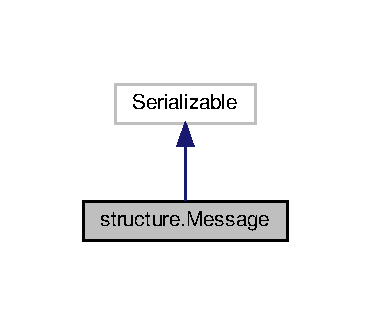
\includegraphics[width=178pt]{classstructure_1_1_message__inherit__graph}
\end{center}
\end{figure}


Collaboration diagram for structure.\+Message\+:
\nopagebreak
\begin{figure}[H]
\begin{center}
\leavevmode
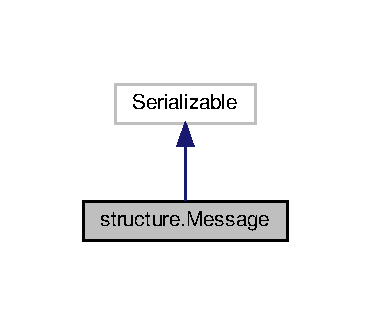
\includegraphics[width=178pt]{classstructure_1_1_message__coll__graph}
\end{center}
\end{figure}
\subsection*{Public Member Functions}
\begin{DoxyCompactItemize}
\item 
\hyperlink{classstructure_1_1_message_a9608c61c1b9a4985db065a86b3e88b10}{Message} (final String author, final String message, final Local\+Time time)
\item 
String \hyperlink{classstructure_1_1_message_a74a4d9d06a57a259434d3a1c8d4305a5}{get\+Author} ()
\item 
void \hyperlink{classstructure_1_1_message_a71321e51a130574d5c3e92b113d38a81}{set\+Author} (final String author)
\item 
String \hyperlink{classstructure_1_1_message_acd0de72e2ae0e0f993b7843c3f5c494c}{get\+Message} ()
\item 
void \hyperlink{classstructure_1_1_message_a1907224cce70e3247d280965bb74b412}{set\+Message} (final String message)
\item 
Local\+Time \hyperlink{classstructure_1_1_message_a851f4b7a16a0f568da25b4a59a9ef4eb}{get\+Time} ()
\item 
void \hyperlink{classstructure_1_1_message_a7e2febd60ee915acad6cdabea44af622}{set\+Time} (final Local\+Time time)
\item 
void \hyperlink{classstructure_1_1_message_a4b7cc15e72f9c4c0cf98c06edea73529}{make\+Time} ()
\item 
boolean \hyperlink{classstructure_1_1_message_a1ed9266f67fed4a68e264d69b219d5b9}{equals} (final Object o)
\item 
int \hyperlink{classstructure_1_1_message_a9d0d32152bd93f3e3bf1f59a5b82b4ef}{hash\+Code} ()
\item 
String \hyperlink{classstructure_1_1_message_a7c4f04f22c5ff83311e33cd54e7f4ce3}{to\+String} ()
\end{DoxyCompactItemize}


\subsection{Constructor \& Destructor Documentation}
\mbox{\Hypertarget{classstructure_1_1_message_a9608c61c1b9a4985db065a86b3e88b10}\label{classstructure_1_1_message_a9608c61c1b9a4985db065a86b3e88b10}} 
\index{structure\+::\+Message@{structure\+::\+Message}!Message@{Message}}
\index{Message@{Message}!structure\+::\+Message@{structure\+::\+Message}}
\subsubsection{\texorpdfstring{Message()}{Message()}}
{\footnotesize\ttfamily structure.\+Message.\+Message (\begin{DoxyParamCaption}\item[{final String}]{author,  }\item[{final String}]{message,  }\item[{final Local\+Time}]{time }\end{DoxyParamCaption})}



\subsection{Member Function Documentation}
\mbox{\Hypertarget{classstructure_1_1_message_a1ed9266f67fed4a68e264d69b219d5b9}\label{classstructure_1_1_message_a1ed9266f67fed4a68e264d69b219d5b9}} 
\index{structure\+::\+Message@{structure\+::\+Message}!equals@{equals}}
\index{equals@{equals}!structure\+::\+Message@{structure\+::\+Message}}
\subsubsection{\texorpdfstring{equals()}{equals()}}
{\footnotesize\ttfamily boolean structure.\+Message.\+equals (\begin{DoxyParamCaption}\item[{final Object}]{o }\end{DoxyParamCaption})}

\mbox{\Hypertarget{classstructure_1_1_message_a74a4d9d06a57a259434d3a1c8d4305a5}\label{classstructure_1_1_message_a74a4d9d06a57a259434d3a1c8d4305a5}} 
\index{structure\+::\+Message@{structure\+::\+Message}!get\+Author@{get\+Author}}
\index{get\+Author@{get\+Author}!structure\+::\+Message@{structure\+::\+Message}}
\subsubsection{\texorpdfstring{get\+Author()}{getAuthor()}}
{\footnotesize\ttfamily String structure.\+Message.\+get\+Author (\begin{DoxyParamCaption}{ }\end{DoxyParamCaption})}

\mbox{\Hypertarget{classstructure_1_1_message_acd0de72e2ae0e0f993b7843c3f5c494c}\label{classstructure_1_1_message_acd0de72e2ae0e0f993b7843c3f5c494c}} 
\index{structure\+::\+Message@{structure\+::\+Message}!get\+Message@{get\+Message}}
\index{get\+Message@{get\+Message}!structure\+::\+Message@{structure\+::\+Message}}
\subsubsection{\texorpdfstring{get\+Message()}{getMessage()}}
{\footnotesize\ttfamily String structure.\+Message.\+get\+Message (\begin{DoxyParamCaption}{ }\end{DoxyParamCaption})}

\mbox{\Hypertarget{classstructure_1_1_message_a851f4b7a16a0f568da25b4a59a9ef4eb}\label{classstructure_1_1_message_a851f4b7a16a0f568da25b4a59a9ef4eb}} 
\index{structure\+::\+Message@{structure\+::\+Message}!get\+Time@{get\+Time}}
\index{get\+Time@{get\+Time}!structure\+::\+Message@{structure\+::\+Message}}
\subsubsection{\texorpdfstring{get\+Time()}{getTime()}}
{\footnotesize\ttfamily Local\+Time structure.\+Message.\+get\+Time (\begin{DoxyParamCaption}{ }\end{DoxyParamCaption})}

\mbox{\Hypertarget{classstructure_1_1_message_a9d0d32152bd93f3e3bf1f59a5b82b4ef}\label{classstructure_1_1_message_a9d0d32152bd93f3e3bf1f59a5b82b4ef}} 
\index{structure\+::\+Message@{structure\+::\+Message}!hash\+Code@{hash\+Code}}
\index{hash\+Code@{hash\+Code}!structure\+::\+Message@{structure\+::\+Message}}
\subsubsection{\texorpdfstring{hash\+Code()}{hashCode()}}
{\footnotesize\ttfamily int structure.\+Message.\+hash\+Code (\begin{DoxyParamCaption}{ }\end{DoxyParamCaption})}

\mbox{\Hypertarget{classstructure_1_1_message_a4b7cc15e72f9c4c0cf98c06edea73529}\label{classstructure_1_1_message_a4b7cc15e72f9c4c0cf98c06edea73529}} 
\index{structure\+::\+Message@{structure\+::\+Message}!make\+Time@{make\+Time}}
\index{make\+Time@{make\+Time}!structure\+::\+Message@{structure\+::\+Message}}
\subsubsection{\texorpdfstring{make\+Time()}{makeTime()}}
{\footnotesize\ttfamily void structure.\+Message.\+make\+Time (\begin{DoxyParamCaption}{ }\end{DoxyParamCaption})}

\mbox{\Hypertarget{classstructure_1_1_message_a71321e51a130574d5c3e92b113d38a81}\label{classstructure_1_1_message_a71321e51a130574d5c3e92b113d38a81}} 
\index{structure\+::\+Message@{structure\+::\+Message}!set\+Author@{set\+Author}}
\index{set\+Author@{set\+Author}!structure\+::\+Message@{structure\+::\+Message}}
\subsubsection{\texorpdfstring{set\+Author()}{setAuthor()}}
{\footnotesize\ttfamily void structure.\+Message.\+set\+Author (\begin{DoxyParamCaption}\item[{final String}]{author }\end{DoxyParamCaption})}

\mbox{\Hypertarget{classstructure_1_1_message_a1907224cce70e3247d280965bb74b412}\label{classstructure_1_1_message_a1907224cce70e3247d280965bb74b412}} 
\index{structure\+::\+Message@{structure\+::\+Message}!set\+Message@{set\+Message}}
\index{set\+Message@{set\+Message}!structure\+::\+Message@{structure\+::\+Message}}
\subsubsection{\texorpdfstring{set\+Message()}{setMessage()}}
{\footnotesize\ttfamily void structure.\+Message.\+set\+Message (\begin{DoxyParamCaption}\item[{final String}]{message }\end{DoxyParamCaption})}

\mbox{\Hypertarget{classstructure_1_1_message_a7e2febd60ee915acad6cdabea44af622}\label{classstructure_1_1_message_a7e2febd60ee915acad6cdabea44af622}} 
\index{structure\+::\+Message@{structure\+::\+Message}!set\+Time@{set\+Time}}
\index{set\+Time@{set\+Time}!structure\+::\+Message@{structure\+::\+Message}}
\subsubsection{\texorpdfstring{set\+Time()}{setTime()}}
{\footnotesize\ttfamily void structure.\+Message.\+set\+Time (\begin{DoxyParamCaption}\item[{final Local\+Time}]{time }\end{DoxyParamCaption})}

\mbox{\Hypertarget{classstructure_1_1_message_a7c4f04f22c5ff83311e33cd54e7f4ce3}\label{classstructure_1_1_message_a7c4f04f22c5ff83311e33cd54e7f4ce3}} 
\index{structure\+::\+Message@{structure\+::\+Message}!to\+String@{to\+String}}
\index{to\+String@{to\+String}!structure\+::\+Message@{structure\+::\+Message}}
\subsubsection{\texorpdfstring{to\+String()}{toString()}}
{\footnotesize\ttfamily String structure.\+Message.\+to\+String (\begin{DoxyParamCaption}{ }\end{DoxyParamCaption})}



The documentation for this class was generated from the following file\+:\begin{DoxyCompactItemize}
\item 
src/structure/\hyperlink{_message_8java}{Message.\+java}\end{DoxyCompactItemize}

\hypertarget{classserver_1_1_server}{}\section{server.\+Server Class Reference}
\label{classserver_1_1_server}\index{server.\+Server@{server.\+Server}}


Inheritance diagram for server.\+Server\+:
\nopagebreak
\begin{figure}[H]
\begin{center}
\leavevmode
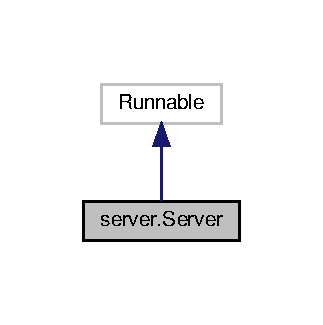
\includegraphics[width=155pt]{classserver_1_1_server__inherit__graph}
\end{center}
\end{figure}


Collaboration diagram for server.\+Server\+:
\nopagebreak
\begin{figure}[H]
\begin{center}
\leavevmode
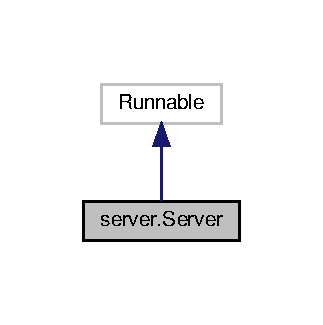
\includegraphics[width=155pt]{classserver_1_1_server__coll__graph}
\end{center}
\end{figure}
\subsection*{Public Member Functions}
\begin{DoxyCompactItemize}
\item 
\hyperlink{classserver_1_1_server_a0cd54beb5f4b2177f7161d2d7d4b6285}{Server} (String IP)
\item 
void \hyperlink{classserver_1_1_server_a803f3b2a096f160a4070a55085f98c2e}{run} ()
\end{DoxyCompactItemize}


\subsection{Constructor \& Destructor Documentation}
\mbox{\Hypertarget{classserver_1_1_server_a0cd54beb5f4b2177f7161d2d7d4b6285}\label{classserver_1_1_server_a0cd54beb5f4b2177f7161d2d7d4b6285}} 
\index{server\+::\+Server@{server\+::\+Server}!Server@{Server}}
\index{Server@{Server}!server\+::\+Server@{server\+::\+Server}}
\subsubsection{\texorpdfstring{Server()}{Server()}}
{\footnotesize\ttfamily server.\+Server.\+Server (\begin{DoxyParamCaption}\item[{String}]{IP }\end{DoxyParamCaption})}



\subsection{Member Function Documentation}
\mbox{\Hypertarget{classserver_1_1_server_a803f3b2a096f160a4070a55085f98c2e}\label{classserver_1_1_server_a803f3b2a096f160a4070a55085f98c2e}} 
\index{server\+::\+Server@{server\+::\+Server}!run@{run}}
\index{run@{run}!server\+::\+Server@{server\+::\+Server}}
\subsubsection{\texorpdfstring{run()}{run()}}
{\footnotesize\ttfamily void server.\+Server.\+run (\begin{DoxyParamCaption}{ }\end{DoxyParamCaption})}



The documentation for this class was generated from the following file\+:\begin{DoxyCompactItemize}
\item 
src/server/\hyperlink{_server_8java}{Server.\+java}\end{DoxyCompactItemize}

\chapter{File Documentation}
\hypertarget{_broadcast_8java}{}\section{src/server/\+Broadcast.java File Reference}
\label{_broadcast_8java}\index{src/server/\+Broadcast.\+java@{src/server/\+Broadcast.\+java}}


Interface do Broadcast\+Impl.  


\subsection*{Classes}
\begin{DoxyCompactItemize}
\item 
interface \hyperlink{interfaceserver_1_1_broadcast}{server.\+Broadcast}
\end{DoxyCompactItemize}
\subsection*{Packages}
\begin{DoxyCompactItemize}
\item 
package \hyperlink{namespaceserver}{server}
\end{DoxyCompactItemize}


\subsection{Detailed Description}
Interface do Broadcast\+Impl. 


\hypertarget{_broadcast_impl_8java}{}\section{src/server/\+Broadcast\+Impl.java File Reference}
\label{_broadcast_impl_8java}\index{src/server/\+Broadcast\+Impl.\+java@{src/server/\+Broadcast\+Impl.\+java}}


Implementa as funções compartilhadas dos nodes.  


\subsection*{Classes}
\begin{DoxyCompactItemize}
\item 
class \hyperlink{classserver_1_1_broadcast_impl}{server.\+Broadcast\+Impl}
\end{DoxyCompactItemize}
\subsection*{Packages}
\begin{DoxyCompactItemize}
\item 
package \hyperlink{namespaceserver}{server}
\end{DoxyCompactItemize}


\subsection{Detailed Description}
Implementa as funções compartilhadas dos nodes. 


\hypertarget{gr_admin_8java}{}\section{src/server/gr\+Admin.java File Reference}
\label{gr_admin_8java}\index{src/server/gr\+Admin.\+java@{src/server/gr\+Admin.\+java}}


Arquivo com as funções do admin do sistema\+:  


\subsection*{Classes}
\begin{DoxyCompactItemize}
\item 
class \hyperlink{classserver_1_1gr_admin}{server.\+gr\+Admin}
\end{DoxyCompactItemize}
\subsection*{Packages}
\begin{DoxyCompactItemize}
\item 
package \hyperlink{namespaceserver}{server}
\end{DoxyCompactItemize}


\subsection{Detailed Description}
Arquivo com as funções do admin do sistema\+: 


\begin{DoxyItemize}
\item quantidade de elementos do grupo
\item o endereço IP de cada elemento
\item a relação existente entre os elementos 
\end{DoxyItemize}
\hypertarget{_server_8java}{}\section{src/server/\+Server.java File Reference}
\label{_server_8java}\index{src/server/\+Server.\+java@{src/server/\+Server.\+java}}


Liga o node server.  


\subsection*{Classes}
\begin{DoxyCompactItemize}
\item 
class \hyperlink{classserver_1_1_server}{server.\+Server}
\end{DoxyCompactItemize}
\subsection*{Packages}
\begin{DoxyCompactItemize}
\item 
package \hyperlink{namespaceserver}{server}
\end{DoxyCompactItemize}


\subsection{Detailed Description}
Liga o node server. 


\hypertarget{_client_tela_8java}{}\section{src/structure/\+Client\+Tela.java File Reference}
\label{_client_tela_8java}\index{src/structure/\+Client\+Tela.\+java@{src/structure/\+Client\+Tela.\+java}}


Arquivo com as funções de construção e interação com a interface do usuario.  


\subsection*{Classes}
\begin{DoxyCompactItemize}
\item 
class \hyperlink{classstructure_1_1_client_tela}{structure.\+Client\+Tela}
\end{DoxyCompactItemize}
\subsection*{Packages}
\begin{DoxyCompactItemize}
\item 
package \hyperlink{namespacestructure}{structure}
\end{DoxyCompactItemize}


\subsection{Detailed Description}
Arquivo com as funções de construção e interação com a interface do usuario. 


\hypertarget{_connection_graph_8java}{}\section{src/structure/\+Connection\+Graph.java File Reference}
\label{_connection_graph_8java}\index{src/structure/\+Connection\+Graph.\+java@{src/structure/\+Connection\+Graph.\+java}}


Arquivo com as funções do grafo de conexões.  


\subsection*{Classes}
\begin{DoxyCompactItemize}
\item 
class \hyperlink{classstructure_1_1_connection_graph}{structure.\+Connection\+Graph}
\end{DoxyCompactItemize}
\subsection*{Packages}
\begin{DoxyCompactItemize}
\item 
package \hyperlink{namespacestructure}{structure}
\end{DoxyCompactItemize}


\subsection{Detailed Description}
Arquivo com as funções do grafo de conexões. 


\hypertarget{_group_node_8java}{}\section{src/structure/\+Group\+Node.java File Reference}
\label{_group_node_8java}\index{src/structure/\+Group\+Node.\+java@{src/structure/\+Group\+Node.\+java}}


Arquivo com as funções do node.  


\subsection*{Classes}
\begin{DoxyCompactItemize}
\item 
class \hyperlink{classstructure_1_1_group_node}{structure.\+Group\+Node}
\end{DoxyCompactItemize}
\subsection*{Packages}
\begin{DoxyCompactItemize}
\item 
package \hyperlink{namespacestructure}{structure}
\end{DoxyCompactItemize}


\subsection{Detailed Description}
Arquivo com as funções do node. 


\hypertarget{_message_8java}{}\section{src/structure/\+Message.java File Reference}
\label{_message_8java}\index{src/structure/\+Message.\+java@{src/structure/\+Message.\+java}}


Classe de mensagens.  


\subsection*{Classes}
\begin{DoxyCompactItemize}
\item 
class \hyperlink{classstructure_1_1_message}{structure.\+Message}
\end{DoxyCompactItemize}
\subsection*{Packages}
\begin{DoxyCompactItemize}
\item 
package \hyperlink{namespacestructure}{structure}
\end{DoxyCompactItemize}


\subsection{Detailed Description}
Classe de mensagens. 


%--- End generated contents ---

% Index
\backmatter
\newpage
\phantomsection
\clearemptydoublepage
\addcontentsline{toc}{chapter}{Index}
\printindex

\end{document}
